\documentclass[onecolumn, draftclsnofoot,10pt, compsoc]{IEEEtran}
\usepackage{graphicx}
\usepackage{url}
\usepackage{setspace}
\usepackage{cite}
\usepackage{longtable}
\usepackage{array}
\usepackage{pdfpages}
\usepackage{wrapfig,geometry,listings,color}
\graphicspath{{./images/}}

\usepackage{geometry}
\geometry{textheight=9.5in, textwidth=7in}

%define code syntax highlighting
\definecolor{codegreen}{rgb}{0,0.6,0}
\definecolor{codegray}{rgb}{0.5,0.5,0.5}
\definecolor{codepurple}{rgb}{0.0,0,0.6}
\definecolor{backcolour}{rgb}{0.96,0.96,0.96}
\definecolor{codekeyword}{RGB}{32,96,160}
 
\lstdefinestyle{mystyle}{
    backgroundcolor=\color{backcolour},   
    commentstyle=\color{codegreen},
    keywordstyle=\color{codekeyword},
    numberstyle=\tiny\color{codegray},
    stringstyle=\color{codepurple},
    basicstyle=\footnotesize,
    breakatwhitespace=false,         
    breaklines=true,                 
    captionpos=b,                    
    keepspaces=true,                 
    numbers=left,                    
    numbersep=5pt,                  
    showspaces=false,                
    showstringspaces=false,
    showtabs=false,                  
    tabsize=2
}
\lstset{style=mystyle}
%%%%%%%%%%%%%%%%%%%%%

% 1. Fill in these details
\def \CapstoneTeamName{		The Cleverly Named Team}
\def \CapstoneTeamNumber{	58}
\def \GroupMemberOne{		Daniel Grocki}
\def \GroupMemberTwo{		Austin Sanders}
\def \GroupMemberThree{		Owen Loughran}
\def \GroupMemberFour{		David Jansen}
\def \GroupMemberFive{		Brendan Byers}
\def \CapstoneProjectName{	Software product life cycle transformation with Docker container technology}
\def \CapstoneSponsorCompany{HP}
\def \CapstoneSponsorPerson{Bryan Crampton}
\def \CapstoneSponsorPersonTwo{Matt MacClary}

% 2. Uncomment the appropriate line below so that the document type works
\def \DocType{		%Problem Statement
				Requirements Document
				%Technology Review
				%Design Document
				%Progress Report
				}
			
\newcommand{\NameSigPair}[1]{\par
\makebox[2.75in][r]{#1} \hfil 	\makebox[3.25in]{\makebox[2.25in]{\hrulefill} \hfill		\makebox[.75in]{\hrulefill}}
\par\vspace{-12pt} \textit{\tiny\noindent
\makebox[2.75in]{} \hfil		\makebox[3.25in]{\makebox[2.25in][r]{Signature} \hfill	\makebox[.75in][r]{Date}}}}
% 3. If the document is not to be signed, uncomment the RENEWcommand below
%\renewcommand{\NameSigPair}[1]{#1}

%%%%%%%%%%%%%%%%%%%%%%%%%%%%%%%%%%%%%%%
\begin{document}
\begin{titlepage}
    \pagenumbering{gobble}
    \begin{singlespace}
        \hfill 
        % 4. If you have a logo, use this includegraphics command to put it on the coversheet.
        %\includegraphics[height=4cm]{CompanyLogo}   
        \par\vspace{.2in}
        \centering
        \scshape{
            \huge CS Capstone \DocType \par
            {\large\today}\par
            \vspace{.5in}
            \textbf{\Huge\CapstoneProjectName}\par
            \vfill
            {\large Prepared for}\par
            \Huge \CapstoneSponsorCompany\par
            \vspace{5pt}
            %{\Large\NameSigPair{\CapstoneSponsorPerson}\par}
            %{\Large\NameSigPair{\CapstoneSponsorPersonTwo}\par}
            %{\large Prepared by }\par
            Group\CapstoneTeamNumber\par
            % 5. comment out the line below this one if you do not wish to name your team
            %\CapstoneTeamName\par 
            \vspace{5pt}
            {\Large
                {\GroupMemberOne}\par
                {\GroupMemberTwo}\par
                {\GroupMemberThree}\par
                {\GroupMemberFour}\par
                {\GroupMemberFive}\par
            }
            \vspace{20pt}
        }
        \begin{abstract}
        % 6. Fill in your abstract    
            	This paper consists of our teams work on this project over the past year. Our project was focused on using Docker and Kubernetes to containerize and improve the servers used for HP's Page Wide printers. This involved detailed design, research, and documentation all of which is documented here. 

        \end{abstract}     
    \end{singlespace}
\end{titlepage}
\newpage
\pagenumbering{arabic}
\tableofcontents
% 7. uncomment this (if applicable). Consider adding a page break.
%\listoffigures
%\listoftables
\clearpage

% 8. now you write!

\clearpage

%%%%%%%%%%%%%%%%%%%%%%%%%%%%%%%%%%%%%%%%%%%%%%%%%%5
% Introduction to the Project
%%%%%%%%%%%%%%%%%%%%%%%%%%%%%%%%%%%%%%%%%%%%%%%%%%%%

\section{Introduction}




This project was requested by Hewlett Packard (HP) to investigate moving printing services used to operate HP PageWide printers into docker containers where they could easily be managed.
HP PageWide printers are large, room-sized printers that are used for 3 different types of printing: corrugated
packaging, high-volume commercial, and sign/display.
They are able to print from 400 to 1000 feet of paper per second with varying levels of quality.
There are many different services that are managed by server stacks which prepare and manage the incoming print jobs.
The work flow for the jobs has many stages and the servers must complete each stage quick enough to keep up with the printer.

These past three terms we finished a project for HP. 
We were tasked with containerizing a micro-service into containers using docker, and then managing those containers with the container orchestration system Kubernetes. 
The micro-service was in charge of managing HP's industrial sized printers. 
They took in PDF's formatted into a way that maximized page space, and ink, before sending the jobs to the printer. 
The micro-service also possessed a front end that existed in a Windows environment. 
This was the part of the program that interacted with the user, and sent jobs to be completed. 
We did not work on the front end of the service. 
The back end, the portion we did interact with and containerize, exists in a Linux environment. 
This is the part of micro-service that is actually in charge of formatting and printing the submitted PDF. 
Both the front end and the back end existed on a server rack dedicated to receiving and  submitting jobs. 
These printers usually print all day, and print thousands of yards of content very quickly so it requires a lot of processing power to make sure pages are prepared for printing at least as fast as they are printed.

This project provided two large benefits for HP. 
The first being that the servers no longer had to be taken offline to update. 
In the past these machines had to be taken completely offline, have the programs stripped from the server, and have the updated programs submitted. 
These servers are often times not connected to the internet and are only on a local access network.
This meant an actual HP technician has to go to the physical site to update it as well. 
The down time meant losing profits for companies, so obviously this behavior is not desirable. 
The benefit of migrating these services was that these machines could run while updating. 
This could be achieved due to the nature of containers. 
When you want to spin up a container, you use a reference image of the container. 
This is basically a recipe for the programs and environment you want to run. 
We can achieve little or no down time by swapping out these images with the updated images while the machine is running. 
As long as the functionality remains constant it doesn't matter what happens inside the code.
The second benefit to our project was we could reduce the amount of racks we need to ship on the server. 
This can be achieved with the container orchestration system. 
The reason they could not reduce the amount before is because they could not run more than one micro-service per rack without there being communication overlaps resulting in bad data. 
Since Kuberenetes comes with their own networks to communicate we could run more than one instance on a rack. 
If we could reduce the number of racks to four, then HP could ship the printer and sever rack in the same container saving the company a lot on shipping.

Our project was sponsored by two HP employees: Bryan Crampton and Matt MacClary. 
They were pretty hands off the entire project. 
They weren't neglectful, but they just promoted an environment to help us learn these technologies. 
We had weekly meetings with them were we would present our current progress and demo code if we had it. 
They would also write and manage sprints on a two week SCRUM cycle. 
Finally they also explained the project to us in a larger scope.

Our team consisted of five members in total: Daniel Grocki, Owen Loughran, Brendan Byers, David Jansen, and Austin Sanders.
Daniel was mostly in charge of the Kubernetes implementation. 
Owen worked on the web sockets and helped with kubernetes as well. 
Brendan handled getting Jenkins and continuous integration/testing up and running for this entire project. 
David worked with PDF box and getting it integrated into the different workers. Austin got the web server prepared and running, along with gradle setup and configuration.  
We all formatted our own docker files for building our codes images.



%%%%%%%%%%%%%%%%%%%%%%%%%%%%%%%%%%%%%%%%%%%%%%%%%%%
% Requirements Document
%%%%%%%%%%%%%%%%%%%%%%%%%%%%%%%%%%%%%%%%%%%%%%%%%%%

\section{Requirements}

\subsection{Change Table}
  
\begin{longtable}{ | m{8em} | m{24em}| m{16em}| } 
\hline
Section&
Original&
New
\\ \hline

4 Specific Requirements&
\begin{itemize}
  \item Contains: "The code being written will model the services that HP actually uses for their printing. It will be written in Groovy with Gradle being used to help with dependencies. These models will then be used for testing the system."
  \item Removed unnecessary descriptions about rollback.
\end{itemize}&
\begin{itemize}
  \item Added: "It is critical that the code written accurately models the services currently being used for at HP. We must show that the communication done by the HP services is able to be properly containerized. Our model system must accurately represent this."
  \item This was added to expand on the how Kubernetes is a tool we are implementing so that these other features are possible, but not that we are implementing said other features, just Kubernetes
\end{itemize}
\\
\hline
4.2 External Interfaces&
\begin{itemize}
  \item "output some statistics and data "
\end{itemize}&
\begin{itemize}
  \item Minor rewording to focus on output logs as source of health
\end{itemize}
\\
\hline
4.3 Functions&
\begin{itemize}
    \item The system will take multiple things as input. The primary input will be new updates to services. Since there are monthly updates, the system will be frequently receiving new images. When it receives a new image, the image should already have been built and successfully ran during the build process. When it receives this image it should then store it in it’s database. When we are ready to push the new image to the client systems, we should be able to push the one that we added to the database. This should eventually output a new update to the containers that are running the services. If there is any errors in the deployment of the updated container, Kubernetes should roll back to the previous working version.

\end{itemize}&
\begin{itemize}  
\item Reworded functions section with more accurate information that is related to the scope of the project removing excess info outside scope.

\item Added description about inputs and outputs to the system prototype as that is what a large portion of our projects is about.

  \item Added more detailed description of Kubernetes "As a whole, the system will also be able to be updated easily because of Kubernetes. The input for Kubernetes are the images of the system that change, and then Kubernetes can manage the deployment with the new images. This results in an output of new containers running in the system. "
\end{itemize}
\\
\hline
4.4 Usability Requirements&
\begin{itemize}
  \item for the rolling update feature of the system. The rolling update should be effective in the sense that they successfully update the images on the client system. Once the images are updated, new containers should be deployed from these images. If there is an issue with these new containers, the system should be able to revert back to the old images. This should increase the efficiency of the entire container update process for the clients. 

\end{itemize}&
\begin{itemize}
  \item Reworded Focus on Kubernetes
  \item There are also usability requirements associated with Kubernetes. Kubernetes is being used to make many features available. Kubernetes functionality, allows for much of the usability requirements for the system to be accomplished. Rolling updates should be possible which allow the ability to gradually release a new image or roll back to an older version.


\end{itemize}
\\
\hline
4.5 Performance Requirements&
\begin{itemize}
  \item Adding
\end{itemize}&
\begin{itemize}
    \item Refocused doc on the fact that the goal was to determine if the prototype could be containerized and put in Kubernetes.
  \item The important metric for performance is if the system will run successfully containerized and in Kubernetes. Since none of these components were built with docker in mind. It may not be possible to fully migrate everything to a Docker and Kubernetes system. Since this system is simply a model of the actually system containerized, it is simply a prototype. Successfully running these services in Docker and Kubernetes is a main metric to determine the success of the prototype.
  

\end{itemize}
\\
\hline
4.6 Limitations&
\begin{itemize}
  \item Removed non relevant rollback features as it is not a feature we implemented but rather a perk to using Kubernetes that we want to allow in the overall system that we created.
\end{itemize}&
\begin{itemize}
   \item Removed Rollback
\item Added info about limited knowledge of actual system for comparison puposes. And how this is simply a prototype of that system
  
\end{itemize}
\\
\hline


\end{longtable}
\clearpage


\subsection{Introduction}



\subsubsection{Purpose}

The purpose of this Requirements Document is to define the expectations of the "Software product life cycle transformation with Docker container technology" project. 
This document will lay out our plans for this project and provide clear specifications for us to follow.
It also provides a clear agreement between us and the client about what is required for this project. 

\subsubsection{Scope}
The purpose of this project is to create a container management system for HPs PageWide Web Press printers. 
The software we create will be a prototype of the system that HP wants to implement on their system.
The goal is to containerize services to utilize less resources on the servers, as well as improve scaling. 
We will use Docker to containerize the services and Kubernetes to manage these containers. 
Our team will start by focusing on HP’s Linux based servers. If our implementation on the Linux servers are successful we will move on to containerizing their Windows servers.
	
\subsubsection{Definitions}
\begin{itemize}
    \item \textbf{Docker:} Open source software platform to create, deploy and manage virtualized application containers on a common operating system\cite{tech}.
    
\item \textbf{Kubernetes:} Open source system used to manage Linux containers across private, public and hybrid cloud environments\cite{tech}.

\item \textbf{Application Containerization:} OS-level virtualization method used to deploy and run distributed applications without launching an entire virtual machine\cite{tech}.

\item \textbf{Docker Image:} A file, comprised of multiple layers, used to execute code in a Docker container\cite{tech}.

\item \textbf{Kubernetes Pod:} Smallest deployable computing units in the open source Kubernetes container scheduling and orchestration environment\cite{tech}.

\item \textbf{Server Operating System:} an operating system specifically designed to run on servers, which are specialized computers that operate within a client/server architecture to serve the requests of client computers on the network\cite{tech}.

\item \textbf{Linux Server:} Linux-based server operating system\cite{tech}.

\item \textbf{Windows Server:} Windows-based server operating system\cite{tech}.

\end{itemize}	

\subsection{Overview}
For this project we will be using both Docker and Kubernetes in order to create our containers for the HP PageWide Web Press. 
Docker is a very popular containerization software, containers are used to package code along with all of it’s necessary dependencies. 
This allows for code to reliably and more easily be ran on different environments. 
Within Docker a container begins as an image which holds the necessary code, run time, system code, system libraries and the settings. 
These images become containers at run time\cite{kub}. 

Kubernetes is an open source software developed by Google that will be used as a way to manage the containers. 
Kubernetes will provide us with way to automate the deployment of our containers, scale them properly, and manage the applications that are developed using our containers. 
Each part of a process will become containerized, what Kubernetes does is throw all of these containers in to something referred to as a pod. 
This pod is pretty much a container that holds a group of containers which allows us to properly manage our entire process\cite{docker}. 

Our primary goal is to containerize the HP PageWide WordPress process on HP’s server stacks. 
Currently HP has two separate server types, Linux and Windows, that we will be containerizing their different services on. 
Our primary focus is on the Linux servers because there are more of them and they contain more of the services. 
As a group we need to figure out how to containerize both HP’s own services and the external services that they use. 
Once we have these services in containers we need to work on getting the containers to properly communicate with each other. 
After the containers are correctly communicating with each other we will use Kubernetes to throw the containers in to a pod and use it to manage the entire process.

Benefits of containing the entire printing process for HP include portability between their different environments, scaling on their server stacks, and no down time for updates. 
Currently HP can only run a single process on each server stack. 
This is because if they attempted to do multiple they would have issues keeping the two processes from interfering with one another. 
One of our goals is to allow two processes to run on a single server stack, with the use of Docker and Kubernetes this should be possible. 
HP will also be capable of updating their services individually when they are containerized. 
Rather than having to take down the entire process each container can be updated on their own. 
This means that there will be no downtime for the entire process because Docker allows you to create a new updated image and swap it out with the current image almost instantaneously. 
If our group is successful in our implementation on the Linux servers we will move on to begin the implementation on their Windows servers.

\subsection{Specific Requirements}

During development, code should be able to be checked into a source control system. 
Docker images for testing must be able to be created from this source code that can locally or a test stack. 
Once source code is ready, it will be committed to the version control tool Git. 
There will be a public GitHub repository to hold the information. 

There will be a continuous integration tool, Jenkins, that will run unit tests on the code and build Docker images. 
Once these images are successfully built, they can be pushed to Dockerhub. 

%mod
The code being written will model the services that HP actually uses for their printing. 
It will be written in Groovy with Gradle being used to help with dependencies. It is critical that the code written accurately models the services currently being used for at HP. 
We must show that the communication done by the HP services is able to be properly containerized. 
Our model system must accurately represent this.

Docker images will be build from the Groovy code written. 
These Docker images must be able to network and communicate with all of the other services that are containerized. 
This includes the networking over TCP as well as HTTP requests.

%new stuff
This networking must also be done in Kubernetes so that we can support many different features of Kubernetes. 
Kubernetes is a DevOps tool that supports many important features such as the ability to create and deploy replicas of our system on the same hardware or rollback functionality.

Once a collection of images has been marked for a software release, they must be testable. 
The entire system must be easily buildable and upgradable for ease of testing. 
The system should allow for brand new images to be added as well as update existing images. 

It is also critical that the services inside of the containers can have their health monitored. 
The services that are containerized have health checks to determine their state and to see if they are working effectively. 
The containers must allow a way to access that information either through Kubernetes looking at the container, or the service inside reporting that information to the system. 

Once the software has been successfully tested, there must be a deployment system for customers. 
It is required that there is a way to deploy the software release with the updated images to customers. 
This must be able to be done in two ways. 
For customers that are connected to the cloud, a remote deploy should be available to them. 
The second way we need to be able to deploy a software release is locally. 
For customers that are not connected to the cloud, there must be a way to manually deploy for the new release locally on site. 
Since Kubernetes is a primarily cloud based solution, setting up the system with Kubernetes will allow this functionality. 

	%REMOVED this is outside of our scope
%In addition, when a new software release is deployed, Kubernetes must implement the rollback feature. This is a built in feature of Kubernetes deployments. If there is an issue, either on a local or remote deploy, the system should rollback to the previous working release and resume without interruption. Remote monitoring of the services is also required here. The status of the services running in the containers should be know and should be able to be monitored by the system. 


\subsubsection{User Characteristics}

There are 3 major groups that will be using this system, they are R\&D, System Test, and DevOps. 
As this technology is still rather new to HP, there is a chance then these groups will not have worked with Kubernetes or Docker before.

%minor rewording
\subsubsection{External interfaces}

This system should allow Development, System Test, and DevOps to interface with the system. Development should be able to produce images and test them in a test environment. Their finished images should get build with a continuous integration tool such as Jenkins. 

System Test should be able to install a collection of images to the system. The system should also be able to output logs about the services running in the containers for System Test engineers to analyze. 

DevOps should be able to deploy the release to the customers over cloud or over a local method. The system should output health metrics for DevOps engineers to look at. 

\subsubsection{Functions}

The system prototype will take JSON input that will determine which PDF is being modified.
The system should support JSON input that will specify all the information about the PDF to be modified.
After the system has preformed its operations on the PDF, it should then store the finalized PDF in the database and be able to fetch it out. 
%added
There are many intermediate functions that are a part of the above function.
There are 3 major services that HP needs containerized.
Each one is responsible for some piece of the PDF modification.
Each one takes some form of input as a JSON string and preforms its changes and passes it on to the next service in the pipeline.

As a whole, the system will also be able to be updated easily because of Kubernetes.
The input for Kubernetes are the images of the system that change, and then Kubernetes can manage the deployment with the new images.
This results in an output of new containers running in the system. 

%old
%The system will take multiple things as input. The primary input will be new updates to services. Since there are monthly updates, the system will be frequently receiving new images. When it receives a new image, the image should already have been built and successfully ran during the build process. When it receives this image it should then store it in it’s database. When we are ready to push the new image to the client systems, we should be able to push the one that we added to the database. This should eventually output a new update to the containers that are running the services. If there is any errors in the deployment of the updated container, Kubernetes should roll back to the previous working version.


%minor wording changes to reflect more kubernetes
\subsubsection{Usability Requirements}

One objective for this system is for it to decrease the amount of hardware that we need to use.
Since this system will be used on actual hardware, making the services more efficient will in turn decrease the resources needed on each physical box.
With the services needing less resources, we can run more services on a single box which should increase efficiency and decrease the amount of actual hardware that is needed. 

%modified to focus on kub
There are also usability requirements associated with Kubernetes.
Kubernetes is being used to make many features available.
Kubernetes functionality, allows for much of the usability requirements for the system to be accomplished. Rolling updates should be possible which allow the ability to gradually release a new image or roll back to an older version.


%for the rolling update feature of the system. The rolling update should be effective in the sense that they successfully update the images on the client system. Once the images are updated, new containers should be deployed from these images. If there is an issue with these new containers, the system should be able to revert back to the old images. This should increase the efficiency of the entire container update process for the clients. 

\subsubsection{Performance Requirements}

%addded
The important metric for performance is if the system will run successfully containerized and in Kubernetes. 
Since none of these components were built with docker in mind, it may not be possible to fully migrate everything to a Docker and Kubernetes system. 
The system we created is simply a model of the actual system that we containerized.
Successfully running these services in Docker and Kubernetes is a main metric to determine the success of the prototype.

Other metrics are that a set of services should take up less resources on a server. 
This means that they should take up less RAM, CPU, and possibly even memory.
In addition the containerized services must run at least as fast as they did before they were containerized if not faster.
Kubernetes must be able to network the containers together in a way that ensures the same level of efficiency as there was before they were containerized. 



\subsubsection{Limitations}

One source of limitations for this system is what HP servers can support.
Since we will be deploying these containerized services to HP’s servers, we must make sure that the servers can support the number of containers we want to spin up on them.
Depending on the size of the containers and any overhead required for their management, we may not be able to put as many containers on a server as we may need or want. 

%added
We will also me limited by the amount of information we can use for performance requirements.
Since our project is a prototype of the actual HP system, we do not have access to the actual data about usage on the physical server.
While we know that containers will use up less space, it will be impossible to say how much more efficient our solution is because our prototype will not be doing as much work as the actual system.
Out solution modeled the communication between services but not the actual performance of the services.

%
%Another source of limitations involves the the rolling updates we plan to implement with Kubernetes. Typically, Kubernetes and Docker make use of cloud services for these rolling updates. With everything living in the cloud, it makes it very simple to push a new update out to all the systems and allow for rollback if there is an error. Kubernetes is designed with this cloud infrastructure in mind and we don’t know how difficult it will be to take advantage of these features if not all of our systems can make use of the cloud. Most of the customer systems that this new container management system would affect not have an issue with a cloud based system. However, some of HP’s customers that would use this can’t support a cloud infrastructure. The features that we can implement with Kubernetes such as this rolling release may be limited by this fact. We will have to determine if we can make use of these Kubernetes features in both a cloud based environment and an older non cloud based environment. 

\subsubsection{Timeframe}

This gant chart outlines the time frame we have in mind for completing each aspect of our project.
\begin{center}
    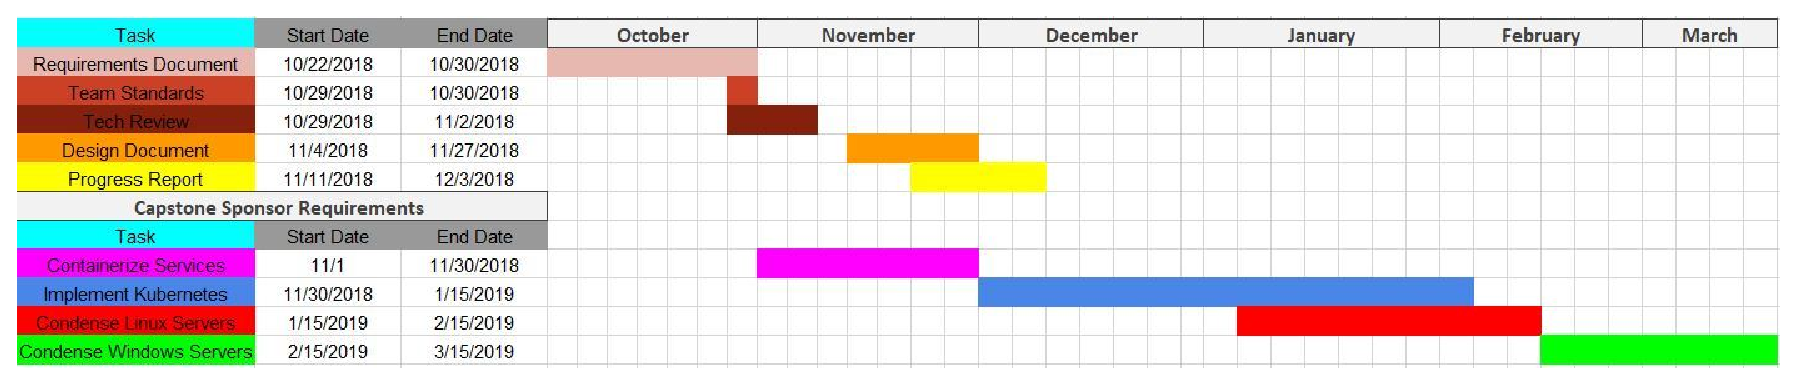
\includegraphics[width=\textwidth, height=5cm]{gant.eps}
\end{center}

\clearpage

%%%%%%%%%%%%%%%%%%%%%%%%%%%%%%%%%%%%%%%%%%%%%%%%%%%%%
%Design document
%%%%%%%%%%%%%%%%%%%%%%%%%%%%%%%%%%%%%%%%%%%%%%%%%%%%%
\section{Design}

\subsection{Change Table}
  
\begin{longtable}{ | m{8em} | m{24em}| m{16em}| } 
\hline
Section&
Original&
New
\\ \hline

2.3 Intended Audience&
\begin{itemize}
  \item Contains: "This document is to serve as guide for the development team to accomplish the project in way that is mutually acceptable between the sponsors and the developers working on the project."
\end{itemize}&
\begin{itemize}
  \item Cleaned up grammar.
  \item Simplified/Removed Wordiness.
\end{itemize}
\\
\hline
2.4 Definitions&
\begin{itemize}
  \item Mentions the use of Artifactory for managing binaries.
\end{itemize}&
\begin{itemize}
  \item Removed reference to Artifactory.*
\end{itemize}
\\
\hline
4.1 System Architecture&
\begin{itemize}
  \item Describes the architecture currently in place at hp.
  \item Mentions the use of Artifactory for managing binaries.
\end{itemize}&
\begin{itemize}
  \item Added short blurb to emphasize the importance of the systems already in place at hp.
  \item Removed reference to Artifactory.*
\end{itemize}
\\
\hline
\end{longtable}
*Artifactory was scrapped due partially to resource issues on an AWS instance but mostly due to the fact that our project did not benefit enough to make deploying it worthwhile.
We ultimately did not have a lot of binaries to work with and the overhead/cost of setting up Artifactory was less than any benefits it would provide.

\subsection{Introduction}

\subsubsection{Scope}

The software outlined in this document is meant to repackage the current software on the servers that control HP’s industrial sized printers.
Our goal is to reduce down time for when printers are updated through constant integration, and reduce the amount of hardware needed by fitting more than one micro-service on each server.


\subsubsection{Purpose}

The purpose of this Software Specification Document is to provide an overview for how the project Software Product Life Cycle Transformation With Docker Container Technology will be designed and executed.
To accomplish this, the document will outline our systems architecture and functionality.


\subsubsection{Intended Audience}

This document is intended for the Sponsors of the Capstone project and the Capstone Instructors.
This document is to serve as a guide for the development team to accomplish the project in a way that is agreed upon with the sponsors.


\subsubsection{Definitions}
\begin{itemize}
    \item \textbf{Docker:} Open source software platform to create, deploy and manage virtualized application containers on a common operating system\cite{tech}.
    
\item \textbf{Application Containerization:} OS-level virtualization method used to deploy and run distributed applications without launching an entire virtual machine\cite{tech}.

\item \textbf{Docker Image:} A file, comprised of multiple layers, used to execute code in a Docker container\cite{tech}.

\item \textbf{Docker Hub:} Similar to GitHub, Docker Hub is a cloud based registry service that allows you to link code repositories, build images and test them.
    
\item \textbf{Kubernetes:} Open source system used to manage Linux containers across private, public and hybrid cloud environments\cite{tech}.



\item \textbf{Kubernetes Pod:} Smallest deployable computing units in the open source Kubernetes container scheduling and orchestration environment\cite{tech}.

\item \textbf{Server Operating System:} an operating system specifically designed to run on servers, which are specialized computers that operate within a client/server architecture to serve the requests of client computers on the network\cite{tech}.

\item \textbf{Linux Server:} Linux-based server operating system\cite{tech}.

\item \textbf{Windows:} A group of operating systems created and maintained by Microsoft

\item \textbf{Riak:} A distributed key valued database.

\item \textbf{Beanstalk:} An open source product that manages job request queues.

\item \textbf{Jenkins:} Jenkins is an automation server that integrates with source controls to automatically build, test and deploy code.

\item \textbf{Websocket:} Instead of streaming data, websockets are built on a message based transport system that is bi-directional.
Both the client and server can communicate to each other at the same time with low latency.
Data is packaged into messages and is reassembled once it arrives at it's destination.

\item \textbf{HTTP:} HyperText Transfer Protocol is a request-response protocol in a client server computing model. It is one method used for processes to interact with each other.


\item \textbf{API:} An API (Application Program Interface) is a set of endpoints used to interact with a software.

\item \textbf{Groovy:} An object oriented programming language built around the Java platform. It can be used as both a scripting language and programming language.

\item \textbf{Gradle:} Gradle is an open source build automation tool. Designed for use with the Groovy language.

\item \textbf{Printing Press:} Printing press is a large machine used to print images and text at high volume.

\item \textbf{MiniKube:} Minikube runs a single-node Kubernetes cluster inside a VM on your laptop for users looking to try out Kubernetes or develop with it day-to-day \cite {minikube}.

\end{itemize}

\subsection{System Overview}

The Software Product Life Cycle Transformation With Docker Container Technology is a project aimed at reformatting HP’s industrial print servers process.
Currently, the servers do not optimize the hardware on board, and when a service has to be updated or changed the entire system has to come offline.
On occasion HP even has to send an engineer to the physical location to apply updates to the machine.
The aim of this project is to alleviate some, if not all, of these issues.

To decrease the downtime of servers while being updated the project will use a combination of Docker and Kubernetes to ‘containerize’ the entire micro service on the servers themselves.
When properly packaged into images the server should suffer no downtime as a result.
This is because images can be removed and updated remotely, and while the micro service is running.
When Kubernetes or another container requests a new instance of that image it can pull the new updated image and swap it out with the outdated image all while the system is running. 
The container will retain the same functionality, just with improved performance.

The second problem that will be addressed in this project is the inefficient use of the server's hardware.
Currently with the micro service running outside of containers it is difficult to run more than one micro service without interfering with each other.
With the use of Kubernetes it would be possible to encapsulate each individual micro service into their own pods, these pods will act as large containers for the entire process.
This way the system could dictate the amount of resources allocated to them.
With this technology in place it would become possible to run more than one instance of each micro service on each individual server.
That means the printer would be able to run on a server with fewer instances of Linux and Windows.

Overall, the goal of the project ‘Software Product Life Cycle Transformation With Docker Container Technology’ is to reduce the downtime of the printers, and reduce the amount of hardware required to run the micro service as a whole.

\newpage

\subsection{Architecture}

\subsubsection{System Architecture}

The system will implement a way for developers to easily develop code and create working images. The dependencies for the developer’s code will be packaged with each docker container. We will be using Git and Github to implement version control. Jenkins will be used for continuous integration with the code pushed to Github. When code is pushed, Jenkins will build and test the code. If this succeeds, we then can take the built image from Jenkins and put it in our image repository. The image repository for this project is Docker Hub. This will contain all the images that we create for this project. In the grand scheme of things, these images will then be able to be pulled by the quality assurance team to test, and the DevOps team to deploy to production. The images on the repository are the images that Kubernetes will be managing. 

It is important to consider how our project will integrate with the current workflow at HP.
Since our project needs to work in their current system, we need to consider the current system in our design process to make sure we are designing it in a way that works.

\begin{figure}[h]
    \centering
    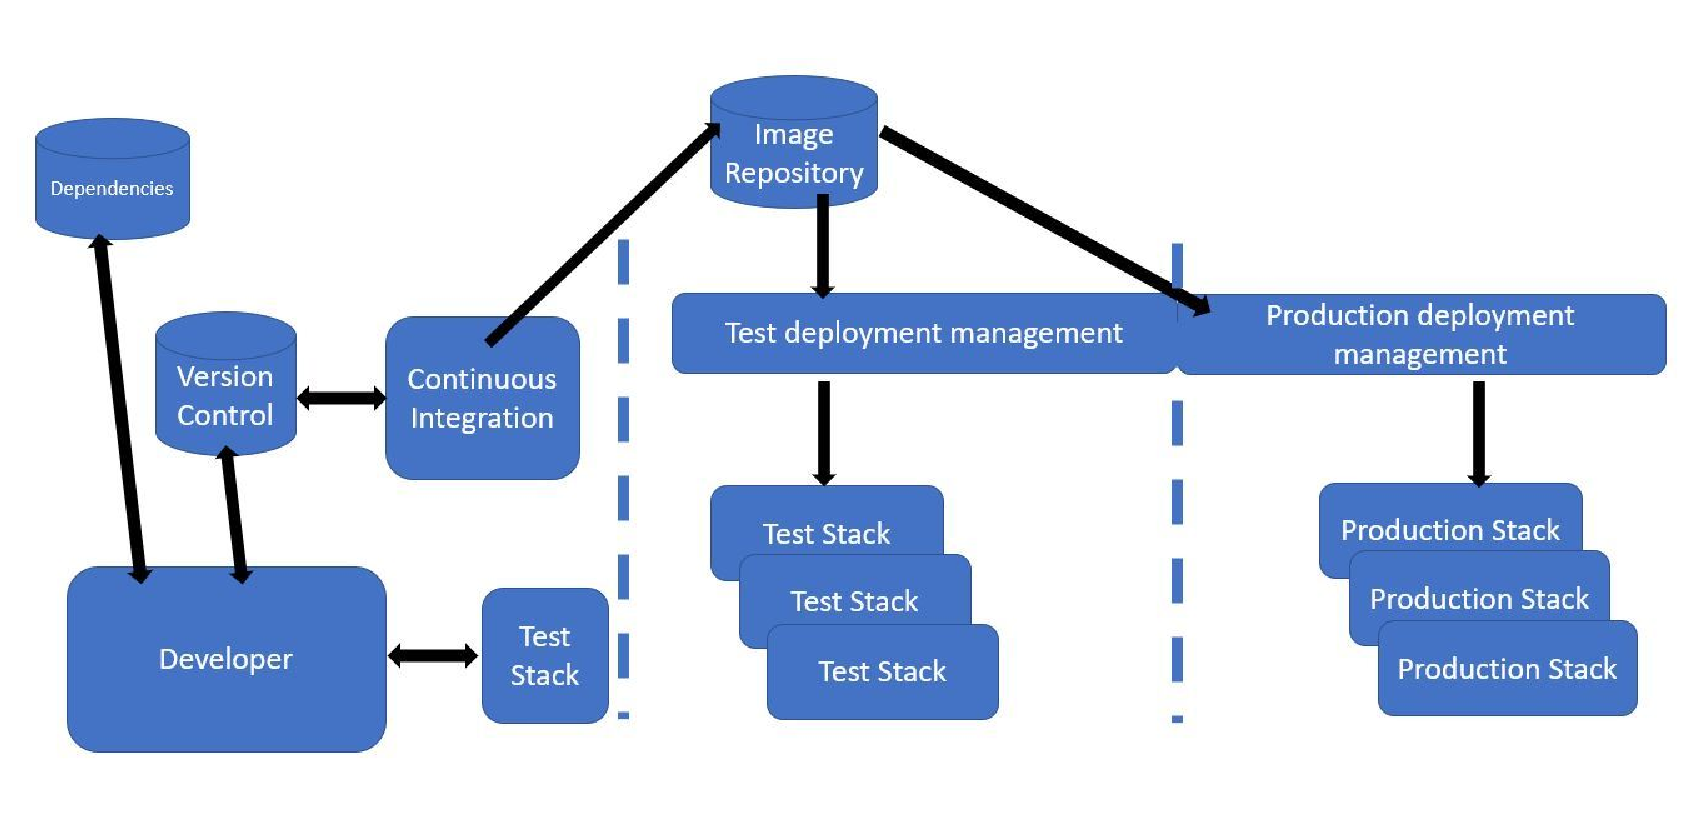
\includegraphics[width=\textwidth, height=8cm]{prjct_arch}
    \caption{This illustrates the workflow we should expect our prototype to experience, when implement it in the current system.}
\end{figure}

\subsubsection{Container Design}

The Linux servers will run containers that will communicate to parse a PDF and prepare it for printing.
There are 5 different containers that we will need: Beanstalk, Riak, WorkManager, WorkerA, and WorkerB.
Riak and Beanstalk are open source projects, but we will need to write the Groovy code for WorkManager, WorkerA, and WorkerB and containerize them.
The parsing and creation of the PDF will be accomplished by the combined work of these processes. 
\newpage

\begin{figure}[h]
    \centering
    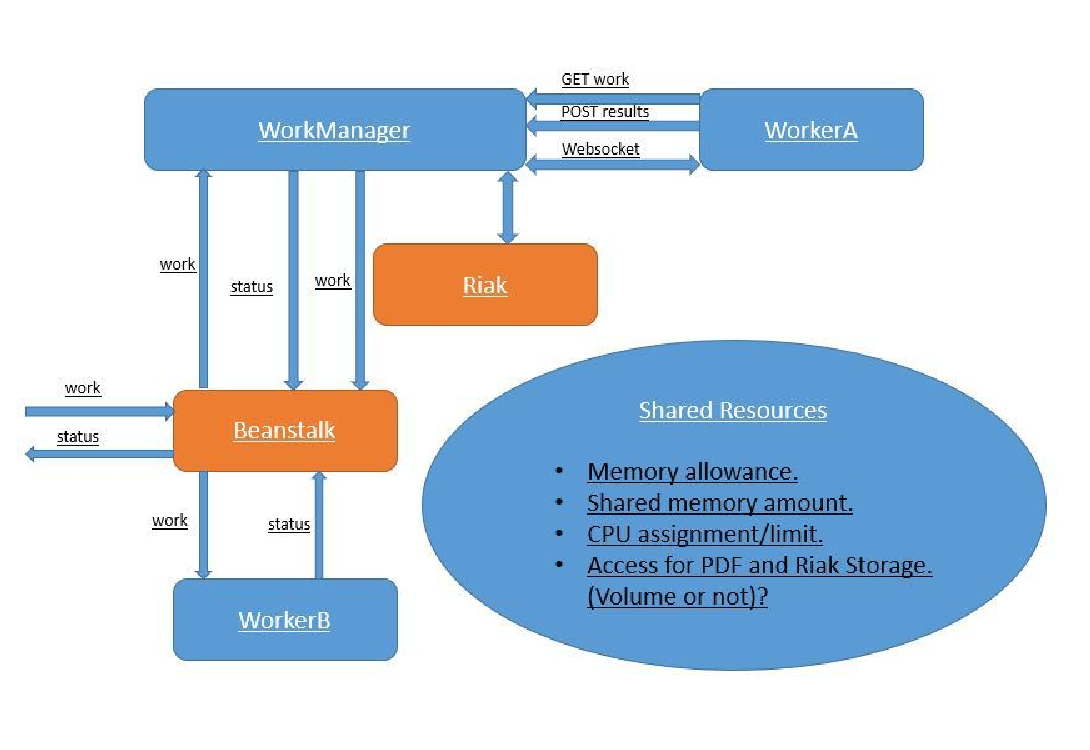
\includegraphics{prjct_arch_workers}
    \caption{The 5 containers will interact with each other in this way. All these containers should share a set amount of resources on the server}
\end{figure}


\begin{itemize}
    \item Beanstalk
    
    Beanstalk is an open source product that is used for queuing up the requests.
    Since it is open source, there is already existing images for it published and we can build off of that.
    It is used to queue up requests for the system.
    These requests can either be new work from the outside or work going from the WorkManager to WorkerB.

    \item Riak
    
    Riak is also an open source project that has already been containerized. Riak will be used to store the final result of the work. After WorkerA and WorkerB have successfully completed their steps, the complete project will be stored in Riak.
    
    \item WorkManager
    
    The WorkManager is the one in charge of managing the Workers. It receives work requests from Beanstalk. It also receives GET and POST requests from WorkerA. It will use a websocket to communicate with WorkerA. The WorkManager will also be responsible for communicating with Riak to store and fetch information. 
    
    \item WorkerA
    
    WorkerA is responsible for inserting content into the PDF that we are trying to print. It will make use of the PDFBox library to do this. 
    It will receive content via a web socket and new work from the work manager. The results are then saved to shared memory with WorkerB. 
    WorkerA sends back a success or failure result to the WorkManager based on whether it was able to successfully add content. 
    
    \item WorkerB
    
    When the WorkManager has received a success from WorkerA, it will then queue up a request via Beanstalk for WorkerB. WorkerB is then responsible for the imposition of the PDF pages. The imposition will involve taking four pages from the PDF produced by WorkerA and putting them on to a larger single page composed of the four pages. This means that it must process the work from WorkerA. WorkerB will access the memory it shares with WorkerA to receive WorkerA’s results. It will then process the work using the PDFBox library and then update the status of the work once it is done. This status is sent back to Beanstalk.
    
    
\end{itemize}

There will be a single WorkManager, but multiple of each Worker A and Worker B as shown in the next picture. All of these Worker A’s and B’s will communicate with the same WorkManager. Once all of these images have been deployed onto a server, we will use Kubernetes to combine them into a pod that only communicates with itself, Beanstalk and Riak. Beanstalk and Riak will have their own pods and will be used by the separate processes because there is no need to make individual copies of them for each process. By doing this, we open up the possibility to running multiple sets of these pods on a single server. Each of these pods will be allocated a certain amount of resources that all the services running in it will have to share. These resources include memory, Riak Storage access, and CPU usage. These pods should not overlap and Workers on one pod should not know about or communicate with a WorkManager on another pod. 

\begin{figure}[h]
    \centering
    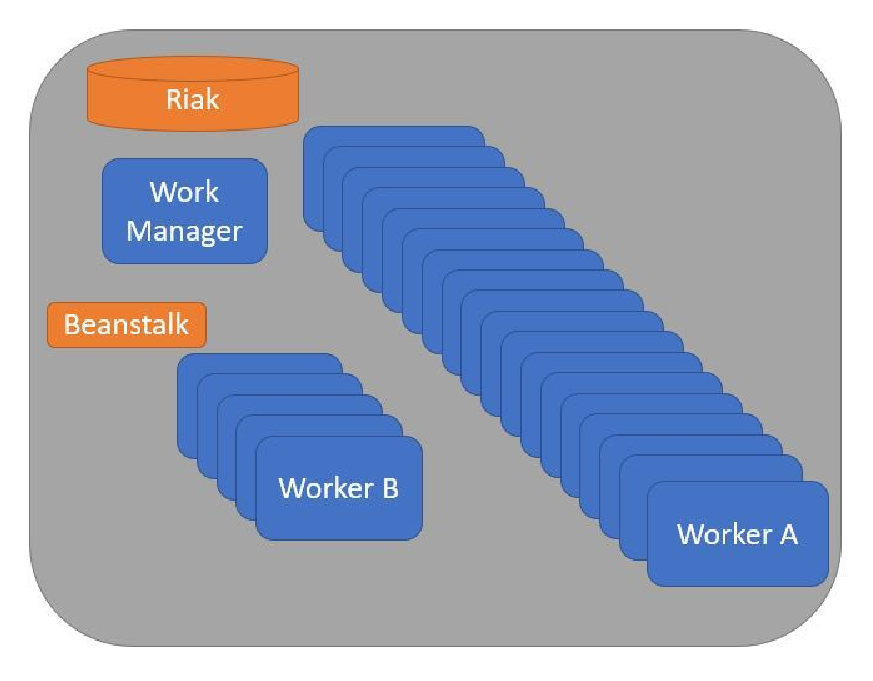
\includegraphics{prjct_arch_pod}
    \caption{There will be multiple instances of WorkerA and WorkerB running in a pod. All of this is considered one pod and must share the same resources and shouldn't interact with any other pod}
\end{figure}

\subsubsection{Design Reasoning}
The system architecture is designed this way mainly to model the existing system. Since everything we are working with is already in production, we must make sure to match the current workflow. We must design our system to fit into their current process of creating updates, testing, and deploying. The fundamental architecture of the Workers must stay the same since we are not changing how they do the PDF parsing. Our goal is to containerize the services to decreases resource consumption. By maintaining the architecture they have for the communication between the 5 different containers, our prototype will be the most accurate and the most useful to HP.

\subsection{Perspective}
In order to satisfy HP our solution needs to be efficient, the main goal with the containerization is to reduce the amount of resources they need to use in order to process print jobs on their printing presses. The perspective section will expand upon the viewpoints we took when designing our solution and choosing technologies in order to achieve this implementation: Context, Composition, Logic, Structure, and Interaction.

\subsubsection{Context Viewpoint}
The context of the project we are creating for HP is essential to the decisions we made. This solution is meant purely to increase HP’s DevOps efficiency and decrease the server costs of supporting their printing presses. The tools we implement will be used by software engineers to deploy and manage their software, and as such flexibility and power will be prioritized over ease of use and simplicity.
\subsubsection{Composition Viewpoint}
The composition of our project is built up of many different components that must communicate with each other in order to form a single process. Within our design we have decided to containerize each individual component, these containers will then communicate with one another. It is very important that each component will be capable of sending and receiving data from it's container. This data must also be sent to and received from the correct components within the process. Once each component has achieved this the entire process will then be containerized. 
\subsubsection{Logic Viewpoint}
The logic behind the design is that it will increase utilization of valuable server resources, it will also allow for less downtime associated with updates and changes to a process. When each component of a process is containerized it allows for individual pieces to be updated without needing to update the entire process. This is done by swapping an old container out with a new updated container. When each process is put in to a container it will allow multiple processes to run on a single server without interfering with one another. 
\subsubsection{Structure Viewpoint}
The structure of our design will require two layers of containers, one layer is a group of containers, the other layer will encapsulate that group of containers. In the first layer each component of a process will be stored in an independent container from the other components within the process apart from Beanstalk and Riak. Inside these containers will be each component and all of the necessary dependencies for it. In the next layer there will be a container for the entire process. This structure will allow for separate processes to run on a single server, it also makes updates and changes to each process much simpler.
\subsubsection{Interaction Viewpoint}
Our design makes it possible for multiple duplicate processes to run on a single server without them interfering with one another. Each individual process is comprised of many different components. Each component in a process is designed to interact with other components within the process in a certain way. It is also important in our design to ensure that components within one process are not communicating with components in other processes on the server. 


\subsection{Docker Component Design}
\subsubsection{Structural Element}
Each component within the printing process will be containerized using Docker containerization technology. The components that will make up the process are all explained in section 3.2. Within each container we will be storing both the component itself and any dependencies that it needs in order to function properly. Each container will also be responsible for communicating with other containers within the process. This means each container must be capable of both sending and receiving data. 
\subsubsection{Design Rationale}
The rationale behind the use of Docker as one of the components within the project is that containerization offers many benefits. One of the main benefits is that containerization can significantly reduce downtime of a process. When a single component needs to be updated or changed Docker allows you to create a new updated container and swap it out with the current corresponding container in the process. This means the entire process will not experience downtime when updating individual components, and any downtime from swapping out a container will be minimal \cite{docker}. 

\subsection{Kubernetes Component Design}
\subsubsection{Structural Element}
Kubernetes is a component that will be used in our project in order to manage our containers. In our case we chose to use MiniKube because it allows us to run Kubernetes locally on our own machines for testing. Specifically we will be looking in to Kubernetes pods in order to encapsulate our entire printing process. Each pod will represent an actual running printing process on the server. These pods will allow us to easily manage our containers as a single entity, it also allows sharing of resources within the pod \cite{kub}. 
\subsubsection{Design Rationale}
The rationale behind the use of Kubernetes is that it will allow us to run multiple duplicate processes on a single server without them interfering with one another. Currently the issue with the non containerized processes is that if you run multiple processes on a single server they may communicate with the wrong process components. This is because the components within the processes are identical to each other, each process will still be responsible for performing a different job though. This means if there is interference from one process to another they likely will not properly complete their job. With Kubernetes we are able to encapsulate each process in to pods. These pods will then perform each process completely independently of one another and there will be no interference's between them. 

\subsection{Jenkins Component Design}
\subsubsection{UI Element}
Jenkins offers a UI element that makes the creation of continuous integration easy. Within this UI we are capable of connecting our Jenkins build systems to different branches of our GitHub. It also allows us to pipeline the containers that are successfully built on Jenkins to our Docker Hub account where the containers will be stored. 
\subsubsection{Structural Element}
Jenkins will mainly be used for unit testing of our containers. When each container is built we will need to test that it is functioning properly using unit tests. These tests will depend on what the purpose of the container is. Jenkins offers us a way to run these tests every time that new code is pushed to our GitHub branches. When code is pushed Jenkins will run the tests we have setup and notify us if they failed or succeeded. If tests are successful the newly built containers will be sent to our Docker Hub account so they are accessible to download and use.
\subsubsection{Design Rationale}
The design rationale behind the use of Jenkins for continuous integration is quite simple, it allows us to know that we are properly creating functioning containers. Jenkins will provide us with significantly less debugging time because it will notify us if our tests have passed or not, every single time new code is pushed to GitHub. This means we will have more time to work on completing the project and spend less time debugging code. It will also make it so our Docker Hub does not get filled with junk containers that don't function properly since the container won't be added unless they pass all tests.



%%%%%%%%%%%%%%%%%%%%%%%%%%%%%%%%%%%%%%%%%%%
% Tech Reviews
%%%%%%%%%%%%%%%%%%%%%%%%%%%%%%%%%%%%%%%%%%%
\section{Technology Review -- Daniel}

%%%%Daniel
\subsection{Introduction}

This tech review document will focus on evaluating different pieces of technology that we need for this project. Our project involves containerizing services used by HP's large scale printers. These containerized services need to be managed in some way and must have a straightforward development cycle. We will be creating this system over the course of this project. By evaluating different technologies for each necessary element of our project, we can weigh pros and cons of each to determine the best choice for the scope of our project. The different aspects of the project that will be evaluated are an option for container orchestration, image hosting, and an operating system for our development environment. For the course of this project, my role will be to help implement Kubernetes and help make sure that our container repositories and development environments are all stable.

\subsection{Container Orchestration}

One piece of technology that we will need is something that will allow for container management. Our project will require the containers that we create to be managed and maintained. This technology should allow us to specify the amount of resources that each group of containers is allowed to use. The system should allow for load balancing of resources to make sure that no cluster of containers is using too much CPU, RAM, or any other resource that is needed. Ideally the system that we choose also is well documented and has a large amount of online help forums. 

\subsubsection{Docker Swarm}
One option is to use Docker Swarm. This is a management system for Docker containers that was created by Docker themselves. This system easily integrates with Docker containers allowing for setup to be rather easy compared to other options. However, this is not as widely used as other options, and we may run into problems that will be hard to research and find good solutions for. Docker Swarm also allows for managing groups of containers via swarms.\cite{d_swarm} It has lost quite a bit of traction due to the popularity of Kubernetes. Despite this, it is still a good solution that would be able to implement all of the necessary requirements. \cite{kub_daniel_tech}

\subsubsection{Kubernetes}
Another option is to use Kubernetes. This open source software allows for straightforward container management. It is the most used solution and is very well documented. It is quite easy to find additional information about problems and solutions. While it doesn't integrate natively with Docker like Swarm does, Docker containers are commonly used with Kubernetes. The setup, while possibly longer than Docker Swarm, should still be straightforward. Also, some teams at HP already use Docker with Kubernetes which means we would have internal support as well. One downside is that Kubernetes suffers from a steep learning curve. It is challenging to set up and requires training and practice to be proficient with it.\cite{kub_daniel_tech} Kubernetes also has pods that allow for a specific amounts of resources to be specified.\cite{kub2}

\subsubsection{Nomad}
A third option would be to use Nomad. This option is a very light version of a container management system. It is designed to have a much simpler architecture than Kubernetes but still provide many of the same services. It is operationally simple and widely available making it a good alternative to Kubernetes. Despite it being simpler than Kubernetes, it still can support large numbers of containers. According to an article examining Kubernetes alternatives by Twain Taylor, “Nomad supports multi-datacenter and multi-region configurations and has been tested on clusters up to 5,000 nodes”.\cite{kub_daniel_tech} This shows that Nomad can support as much as Kubernetes can. However, the fact that Nomad is so simple means that it won't have as many features built in. It may take more work to get everything we want working on it. It would likely take much more set up to get recourse management on par with the other options.

\par
After looking at these different solutions, Kubernetes appears to be the best all around solutions. The biggest reason for this is because of its wide usage. Since it is the most used approach, this means there is lots of documentation and resources to help get set up and solve problems. In addition, we will have resources from HP, since they already use it. Kubernetes will be much more difficult to get initially set up than Swarm; however, the large amount of support will make up for it. Kubernetes is a better solution than Nomad since we want more than the bare bones for a project that is primarily based around managing containers. 



\subsection{Container Repository}
For this project, we need a place to host the images that we have built with Jenkins. The images should be able to be pushed there by our continuous integration tool after the unit tests have passed. It should also allow for easy access to the images for us to pull them and use them to make containers. We also want a hosting cite that is relatively inexpensive as our project is mainly geared as a prototype. There are several different image hosting repositories that we could use. 

\subsubsection{Docker Hub}
The most standout example is Docker Hub. As it is hosted by Docker, it has very easy integration with the Docker images. It is similar to Github in the fact that you can make repositories and add collaborators to them. It also integrates very well with Gihub and Bitbucket, two of the largest code repository services. It also allows for automatic builds to be linked to these repositories. This is very important when using some sort of continuous integration tool. According to \textit{Comparing four hosted Docker Registries}, it has the downside of some performance issues with large amounts of traffic.\cite{docker_hosting} Docker Hub does have the advantage of being very inexpensive and the pricing is based on your usage. 

\subsubsection{Quay}
An alternative to Docker Hub is a product produced by Red Hat. Quay is a container registry that allows for secure storage and deployment of containers. It is able to automatically scan for vulnerabilities in the containers hosted on it. It allows for integration with continuous integration tools as well. Teams can be created to provide access to the repositories for everyone that needs to work on it. This product comes with many features, however it is not free as it is produced by Red Hat.\cite{quay}

\subsubsection{Artifactory}

The third option we could use is Artifactory. This is a repository manager that is geared towards larger corporations. It is an open source product, which means that it will have quite a bit of community support. Another advantage of this product is that Artifactory can be used for things other than container management. For example, HP already uses it to help manage dependencies for projects. It also allows for continuous integration with Jenkins as HP already uses it for that. However, the downside is that using it as a container management system is expensive. \cite{docker_hosting}

\par

Despite HP already using Artifactory, the price to host containers on it seems a little steep. It would be nice to have the easy integration with their existing system, but it doesn't seem worth, or at least not worth for the scope of this project. For similar reasoning, Quay doesn't seem like the best option either. This leaves Docker Hub. While Docker Hub doesn't have as many features as the other systems, it is relatively inexpensive and possibly free for the scope and size of our project. Docker Hub also has the advantage of easily integrating with Docker images.


\subsection{Development Environment}
For this project, we must determine what our development environment will look like. Our client has requested that we choose an operating system that all of us will work on for this project. This is important as we want everyone to have the same development environment. Having the same development environment will make the entire process much smoother as we won’t have to worry about compatibility issues. Docker is able to run on Windows and Linux, however there are differences in how it is set up. We don’t want any of these differences to affect the containers that we are running and creating. Since we plan on implementing the Linux side of things first, we can eliminate Windows as an option for a development environment. However, we may need a Windows installation towards the end of the project when we work on containerizing those services. Until then, we need to choose a good Linux distribution to use. HP currently runs Red Hat Enterprise Linux on their servers that run the services we are containerizing. It would be ideal to choose this flavor of Linux, but we are unable to install it without paying money for it. For our local machines during the project, we have to choose our own Linux distribution. We ideally want an environment that is similar to Red Hat. It would also be nice to have a well supported operating system with many users and one that is stable so we don't have to constantly update it.

\subsubsection{Ubuntu}
One option would be to use Ubuntu. This is one of the most common and user-friendly Linux distributions. It is very easy to install and has a lot of community support for it. This distribution of Linux is based off of the Debian system.\cite{rh_vs_deb} It is a very stable distribution and has long term support. The fact that Ubuntu has a lot of support would make it a good choice for the project. Unfortunately, it is not as similar to Red Hat which is a disadvantage compared to other choices.  

\subsubsection{CentOS}
Another option is to use CentOS. This distribution is based off of Red Hat. Since we are unable to get access to Red Hat Linux, trying to get as close to it as possible is a very good idea. This gives it a distinct advantage over Ubuntu, since Ubuntu is not. CentOS, like Ubuntu, is rather stable, so we do not need to worry about needing constant patches or worry about things breaking. It should work just fine right from install. Due to it's similarities to Red Hat, most of the online support involving Red Hat could also help us.\cite{rh_vs_deb} 

\subsubsection{Fedora}
A third option worth considering is Fedora Linux. Like CentOS, Fedora is a branch of Red Hat Linux. Fedora has updates approximately every 6 months.\cite{cent_vs_fed} It is constantly changing and has a lot of new improvements over the previous versions. These updates provide plenty of valuable features and functionality. However, the downside of numerous updates is that it could possibly break something. We could run into errors or problems while we are developing. Ideally, our development environment would be secure and unchanging. With Fedora, we run the risk of a feature causing a security vulnerability which may require us to update our environment which could cause other issues. \cite{cent_vs_fed}

After looking at all of the choices, CentOS appears to be the best option. Since we plan on developing the Linux side of things first, Windows isn't the best option. We want to develop Linux containers on a Linux machine. Since HP currently uses Red Hat, CentOS seems to have a clear advantage over Ubuntu. While Ubuntu is simpler to install and has a lot more built in features, it’s architectures is not as similar to Red Hat as CentOS is. CentOS, is in the same family as Red Hat which makes it a good choice. It also beats out other flavors of Linux in that family such as Fedora. Fedora, while similar to Red Hat, is much more cutting edge. It has many more features, but it is more unstable which introduces a lot more variables to worry about. CentOS keeps things simple and close to the distribution that HP currently uses on their servers. Since all of these OS's have large amounts of community support, finding help for the one we choose shouldn't be an issue.

\subsection{Conclusion}
By looking into different tech options for each piece of technology we need, we can determine the best options for our project. For container orchestration, Kubernetes is the best choice. It has a large amount of online support and we also have internal support from HP. For an image hosting cite, Docker Hub is the best choice. It is the cheapest option and it has easy integration with continuous integration tools and Docker images. For our development operating system, we are choosing CentOS. It is the closest Linux distribution to Red Hat which is what the HP servers run. It is also stable and we won't have to worry about constant updates. By looking at all of these different options, we have found the best choices for our project to be the most successful. :



\section{Technology Review -- Owen}
\subsection{Introduction}
    HP must build and deploy a vast collection of software applications and websites for their commercial printing press. They are looking to optimize the process in order to maximize their efficiency, and in turn reduce costs. Specifically, they are curious about the possibility of containerization on a large scale for testing, development and deployment of their printing press software. This leaves our capstone project with a task: research the containerization solutions available, implement and test them on a small subsection of their utilities before ultimately bringing them to scale. Our goal will be to determine if it is worth HPs time to expand on containerized development, meaning we must show it is cost effective and will improve their efficiency.

    In order to accomplish this our group will make use of many different technologies working together one with another to create an in depth and complete final product. I will be focusing my technical research and skills on what programming language we will use as well what tools we will use for package management and version control. Specifically I will be comparing between: Groovy, Java Spring, and C\# for the programming language, Git, SVN, and Mercurial for our version control, and Gradle, NPM, and Pants for our package management.

\subsection{Programming Languages}
\subsubsection{Groovy}
Groovy is an object-oriented programming language based upon java, it has many modern day features and can be used for either compiled or scripted programs through the Java Virtual Machine. It is fully compatible with standard java syntax and can take advantage of any java library. You can often simply use straight Java code and still have compilation success. However Groovy is not just a clone of java, it can be built and ran with less dependencies than java itself, giving it the option of being more lightweight and compact. Being so strongly compatible with java itself will make this language easy to pick up for anyone who is familiar with the syntax of Java. Furthermore groovy also adds some features such as: static/dynamic typing, operator overloading, associative arrays, regex support, string interpolation and more. Most import to our project is the modularity of Groovy, being able to cut and groom the language down to do exactly what we need it to be and nothing more is vital to having an effective implementation of containerization. Additionally we may take advantage of the fact that Groovy can also be used as a scripting language in order to design some portions of our project. Sadly there is not very much of a community behind this language, as it seems to be dying out.
\subsubsection{Java Spring}
Java Spring is a framework for Java, created with the goal of being highly scalability for enterprise needs. Java Spring is even more compatible with standard java than Groovy as it just adds different modifiers and alternative ways to more efficiently complete tasks for web based applications. Java Spring is very common in the industry and thus has lots of documentation and support allowing for us to easily research ways to implement what we need. However; Java Spring is primarily marketed as being a tool for building API's with, and while we will be doing some API work this does not fall under the bulk of the project. The decorators in Java Spring can also get fairly complex, possibly making it difficult to fully utilize what Spring has to offer. Regardless Java Spring is incredibly prevalent in industry right now, and it may be worth using for the project solely so that we can become more familiar with it.
\subsubsection{C\#}
    C\# is Microsoft's take on a modern backend language, differing from the other two options C\# is actually based upon C, and follows the Common Language Infrastructure. Some features of C\# include: strong typing, automatic garbage collection, and bounds checking. C\# is meant to be portable and accessible to everyone in the world, applications built on it should be usable on any modern system. The language is efficient at memory management and fairly lightweight compared to Java Spring though not as efficient as C itself. C\# has numerous libraries to pull in from in order to accomplish various tasks and has a large set of documentation and community behind it to show support.

\subsubsection{Table}
\begin{table}[h]
\begin{tabular}{|l|l|l|l|l|l|}
\hline
            & JVM & Modular & Prevalent in Industry & Scripting Language & Common Language Infrastructure \\ \hline
Groovy      & yes & yes     & no                    & yes                & no                             \\ \hline
Java Spring & yes & no      & yes                   & no                 & no                             \\ \hline
C\#         & no  & no      & yes                   & no                 & yes                            \\ \hline
\end{tabular}
\end{table}
\subsection{Version Control}
\subsubsection{GIT}
    Git is the prevalent version control software used today, it was originally developed by Linus Torvalds the creator of linux. Git is based upon distributed architecture, and is a Distributed Version Control System. This means that every developer using Git for a project has the whole project history on his locale repository, and that no single server holds all the project history. Git was designed to work quickly, securely, and with power. Git does its versioning based on file contents not file names, meaning renaming a file will not flag a change block. Being distributed, Git allows a user to be working on a feature update, but quickly switch back to a current version in order to do a bugfix, all on a locale machine.
\subsubsection{SVN}
    SVN is the less popular centralized version control system developed by apache. Being centralized means that unlike Git it requires a connection to a central repo. Meaning that the user pulls down a copy of the project files onto their machine, and anytime they want to make a commit they must push it up to server. No connection to the server means no commits. SVN has no automatic merge conflict resolution when multiple users are commiting to a repository. Due to these reasons we will not be considering SVN for our version control.
\subsubsection{Mercurial}
    Mercurial is much like git, it is distributed so we don't have to worry about the issues that come up with SVN's reliance on a central server. Mercurial was released within one month of Git, and has numerous features that are meant to make it easier to transition to from SVN. Compared to Git mercurial is very inflexible, but does this for the trade of a highly organized system that relies on only one binary file to function (git has 144). Otherwise the two softwares are very similar, Mercurial leaning towards the strict and slow, but organized and exact, with git being fast and flexible, but spread out.
\subsection{Package Managers}
\subsubsection{Gradle}
Gradle is an open source build automation system similar to apache maven, it was built with multi-project builds in mind. This means that it is capable of bringing together projects from multiple teams to form a compiled and built final product that can be extensively tested and deployed. It is able to build modularly, meaning that it can determine which parts of the build have changed and need to be rebuilt. Gradle was initially developed for Java, Groovy, and Scala, meaning it will support our choice of Groovy.
\subsubsection{NPM}
NPM is an open source javascript package manager, it comes preinstalled with Node.js. And is primarily built around a command line client. The client interacts with a remote registry of packages to pull them in and install them into a given directory or project. It also manages all local dependencies so that one can be sure there software will run the same on any developers machine. Sadly it is not powerful enough for our needs, nor does it function with our desired programming language.
\subsubsection{Pants}
Pants, similar to Gradle is designed for large codebases, it allows for very exact dependency management and is both scalable and modular. As opposed to Gradle which builds upon Maven, Pants was built from the ground up. Pants take advantage off a concept called a Monorepo, which allows for it's scalability through increased code reuse, easy collaboration, refactoring instead of working around, and powerful dependency management. Pants supports Java, Scala, Python, C/C++, Go, Thrift, Protobuf, and Android code, and while it does support Groovy through plugins it's support is just not enough for our project.
\subsection{Conclusion}
So after my research I have decided that we will be using Groovy as our primary programming language due to its modularity fitting well into the lightweight product that we desire, and it's ease for us to pick up coming from java backgrounds. For version control we will use git as we are all already well versed, and due to its flexibility and prevalence in industry. We will also be using Gradle for package management and building our application, it fits perfectly with our other choices and seems to be powerful enough to get the job done.

\newpage

\section{Technology Review -- Austin}

\subsection{Introduction}
For our senior project we are working software for one of HP’s industrial size printers. The HP PageWide T400S Press. This printer is capable of printing 11,640 square meters of paper or corrugated cardboard an hour. This printer is used in an industrial setting where the consumer is trying to maximize the amount of material they can process in one day, so any delay in printing would cost the company money and they do not like it when that happens. A printer this size takes a lot of printing power to run and manage. In fact it ships with an entire server rack. 

Depending on the model the company buys the server will ship with two windows server shelves and 2-15 Linux based server shelves. These server shelves run something called microservices. Instead of one large process on each server rack the tasks the server has to complete are broken down into small individual services. Each individual service is grouped into their respective task they complete. Then every time a service needs a task completed they will spin up an individual instance of that process. This makes it so some groups of services sometimes have upwards of 16 instances of itself running at once. While the program is broken down into microservices the entire collection, or fleet, of microservices are working towards completing one larger unified goal. The Linux based servers are in charge of taking the pdf sent into the machine and turning it into something the printer can understand. This part of the project isn’t ours, but it is a bunch of complicated and difficult math like linear algebra, vector calculus, and anything else that can help modify an image on a computer. The windows server is in charge of communicating between the Linux servers and the printer itself. The windows server would take in a pdf of the image the consumer wants to print. It would then hand the image to the Linux servers. The linux servers would work their magic, and perform the complex math to format the pdf into something the printer can understand. Once the linux server has formatted the file correctly the windows server will then take that information and send it to the printer. The printer with an image to print and a quantity will then print out the appropriate amount of images for the consumer. It is a pretty involved and nifty process to operate a multi-million dollar piece of machinery.

Now for the part where our project comes in. As right now each fleet of services run independently on their individual server shelves. This creates a few problems that we are hopefully going to solve. The biggest issue is updating the server rack. When we want to update a server rack currently best case we need to take the individual server rack offline while it is updating, and at worst we need to take the entire server and printer offline. This cuts into HP’s technicians time, and cuts into company profit margins while it is offline. This is a big turn off for companies that are looking into printers to purchase. The second problem is each server rack has enough processing power to run at least two fleets of services. 

These problems can be solved by migrating all of these services onto docker, managing them with kubernetes, and ensuring high quality software with Jira. We could port all of the services onto docker images. This means everytime a service needs another service they can spin up a docker image. This comes with another advantage of continuous integration. Meaning everytime we want to update the server we can just upload the updated images to the machine and delete the old ones once the new images have been run and work. This could even be done while the server is completing a process. This would save a lot of money and time for the company and for us. We could then isolate and manage each microservice with kubernetes. This would allow us to hypothetically run multiple microservices per server and simultaneously reduce the amount of racks we need on the entire server. Finally we would implement Jira to test code every time we push a new branch to master. When it is pushed to master it is run against a bunch of unit tests, if the new branch fails any unit tests it is rejected and not integrated into master. This ensures only high quality code is submitted to the master branch. There of course would be other fail safes on board the printer and server, but this is just another form of quality assurance on board.

\subsection{Containerization}

The first technical piece we have to deal with is the containerization software we want to use. Containers are neat little environments we can package software into. We put everything a process needs to run into one container and plug it into the Kernel. The advantage to this is the program has everything it needs. It doesn’t need to get libraries, access storage, etc. Everything it needs to execute is right there which cuts down on resources used and storage. 

The packages are stored in neat little containers called images. Once the service is needed the image is retrieved and is spun up. Once it is running it is considered a container. From one image multiple containers can be spun up. This is extremely useful because some of our microservices needed to be called up to sixteen times in one instance, so we need to be able to spin up multiple containers. The next advantage is we can plug in and plug out images on the fly. Mid Execution we could pull out an old image and update it with the new one. Since it has the same functionality it will spin up the new updated image as if it was the old one and continue execution. This would allow for seamless integration. Since containerization gives us so many advantages we need to be careful in our selection of a service, so it can perform well.

\subsubsection{Docker}

The most prominent containerization tool on the market currently is Docker. Docker is an attractive prospect because it is the most popular container service and with that comes with immense community support. This means that people are working on this open source project continuously adding features and fixing bugs. On top of the technical support since it is the most used it is far easier to find solutions to bugs with this software. Since it is so popular someone somewhere else probably had the same problem.

On top of all of that it is the most complete docker service currently. Large companies like IBM and Red Hat also contribute to this projects source code. This ensures a solid code base and making it a very viable option.

\subsubsection{Core OS rkt}

Another option is Core OS rkt. This iteration of container technology comes with a few perks. It is built directly on systemd, which builds the entire kernel, which means it is running about as low as something can run. This means you would be communicating directly with the hardware on the machine. Making it light and quick. There are some drawbacks with this decision though because since it is built to run on systemd this means it is only viable on linux systems. This would be fine for about 80\% of the project, but there are two servers that run windows that we need to be concerned about.

\subsubsection{LXD}

One final good option to consider would be LXD. The company behind ubuntu, one of Linuxes most popular and accessible flavors, created this container service. These devices plug right into linux sockets on run there. They have some advantages like security. It is much easier to manage permissions from the socket so no malicious users would be able to access them.

Their API is intuitive and well documented making interaction with the containers painless and easy. They are scalable. There is no real end to sockets, so you can have thousands of node connected to containers running at the same time. However again the biggest drawback is that this only runs on Linux making the windows implementation difficult. Windows is again the downfall to another great software.

\subsection{Container Management}

The second obstacle to tackle is managing all of the containers. This technologies goal is to manage an entire microservice of containers. If we could get even two microservices running on one server shelf without them interrupting each other that would cut down on the cost the consumer needs to spend on buying a printer because we would be able to cut down on the hardware.


\subsubsection{Kubernetes}

Kubernetes was developed and funded originally by the big dog himself: Google. This means the code base will be strong and the features should be intuitive. Kubernetes fits our bill well because we are allowed to group services into things called pods. The pods are essentially microservices. They are collections of containers that the software can control. We can control them through an API the software provides and we can update and modify them as we see fit. Kubernetes can also fit onto any system that can fit docker so we would not have to worry about porting any functionality.

\subsubsection{Docker Swarm}

Now docker swarm would be another extremely attractive solution. Mainly because it is endorsed and supported by docker itself. Since our project is going to be using docker having a service that is already supported would be nice because it means there will be fewer strange errors to deal with. However the big drawback of Docker Swarm is the support seemingly ends at the 'swarm'. This means that we can manage one microservice well, but we cannot manage more than one. We could run multiple instances of docker swarm, but then we might have a collision of system resources. This hang up makes docker swarm not as viable of an option.

\subsubsection{Apache Marathon}

Apache Marathon is also another nice option. Apache delivers a suit of well designed and robust software. It is another docker orchestration software that is capable of combining all of our services into one larger service. It has a complete REST api and an intuitive set of features. However the drawbacks come at the fact that it is designed for higher level applications like web servers and other similar technologies.

\subsection{Software Tracking}

The final technology we need to concern ourselves with is the automation server. The job of the automation server is to continually check the code we push to the master branch. Everytime we attempt to merge a branch or push changes to a branch the automation server will run the new code against all of the unit tests to see if it meets the standard of the previous code. If it fails any unit tests then the changes are rejected, and the software engineer is notified. This ensures that all of the code pushed to the master repo is always up to the same standard, so we don't send broken code out to any of our consumers.

\subsubsection{Jira}

Jira is the current standard at HP and the build automation tool they currently use. Jira is nice for several reasons. It can help with long term projects because it can track the project and its individual tasks for the team. It can also help the team manage their time, and use it appropriately so they don't misuse any of it. It can also gather information on work flow to hopefully optimize the development of the project. 

The main issues are typical of any software. Sometimes the process become unresponsive and it is difficult to recover from a partially built repo, and other small bugs. Another large complaint is that comments for code are viewed chronologically so sometimes it is difficult to have context on what they were explaining.

\subsubsection{Jenkins}

Jenkins is another build automation with a lot of benefits. It allows for continuous integration which can make testing go faster and less painless. On top of that it can also deploy working code to the related servers for you, so even once it has tested the software it can also send it to the appropriate place. It has a lot of services since it is an open source software. It can manage database schema, set up command line scripts for testing, etc. It also has plugins to help with the utility of the service.

However the biggest drawback is the fact that is open source. Open source is a double edge sword. Since many people are working on the product it is hard to ensure the quality that you would be able to at a company. Because of this once you hit a wall with the service you can: open a ticket to fix it and wait, or find a work around. The service is vast, but since it is open source once you hit a wall you hit a wall. That is a dangerous variable to have.

\subsubsection{Maven}

Maven is cool because it almost acts more like gradle. It can plug into verison control systems and manage projects. On top of that it can also handle dependencies for the project and make sure your code has everything it needs. Due to this Maven is more of a small scale software and does not fit the scope of what we need from the service.

\section{Technology Review -- David}
\subsection {Introduction}
    My role in this project will consist of three things containerization, continuous integration and build tools. Currently we have decided to use Docker as our containerization tool, Jenkins for continuous integration, and Gradle for our build tools. Within this document I will explain what containerization, continuous integration, and build tools are. I will also explain why we chose the tools that we did, over the other tools available, and how these tools will help us complete our project.
\subsection{Containerization}
    Our project is focused on making the HP printing process for their PageWide Web Press' easier to update without downtime, take up less server space, and not interfere with other processes on the same server stack. We are working on their Linux based servers, each server currently has a single process running on it. These processes are composed of a large list of services. One solution we have come up with is containerizing each service with Docker. Below I will explain the current process, as well as give an alternative option to Docker. I will also explain why Docker is our best solution.
    \subsubsection{Current Process}
    In order to understand why we are looking to containerize HP's PageWide Web Press it is important to understand the current process, and also compare it to alternatives. There is a chance that we end up implementing our project and find out that the current process is better. Within the current process there is no containerization or virtualization in any part of the process. Each Linux server at HP runs one single process comprised of many different services. These services all need to speak to each other in order to function properly. Because there is no virtualization or containerization, it is not possible to run more than a single process on each server or else they will interfere with each other. This is because there is nothing that will make one process be recognizable from another since they are duplicates of one another. The only benefit of this implementation is that it is very easy to implement. There are some major negatives to this implementation, such as server space and updates. In this implementation there can only be one printing process running per server, which means that each server has unused processing power that is pretty much going to waste. Another negative is that when you update any service, in the current implementation, you have to stop the entire process, not just the service you are updating. This leads to a lot of down time. Overall the current process is not a good solution to our problem.

    \subsubsection{Vagrant}
    One possible solution to the containerization issue is to use Vagrant. Vagrant is an open sourced tool for creating and working with virtual development environments, these environments are usually virtual machines \cite{vagrant}. Vagrant offers multiple benefits to the HP PageWide Web Press process. These benefits include the ability to update each service of the process individually, as well as possibly running multiple processes on a single server stack at the same time. Because each service within the process will be running on it's own virtual machine, you won't have to stop the entire process when you want to update a single service within it. Instead you can stop that single service, update it and start running it again, minimizing downtime. Everything is virtualized so it will also make it easier to run multiple processes on a single server stack as they will be less likely to interfere with one another. One issue is that each virtual machine has it's own operating system that comes with it, so it takes up a lot of memory for each service \cite{VagvDoc}. This means that this may not actually be a good solution to the problem we are facing.
    
    \subsubsection{Docker}
    We decided the best solution for our problem is to use a containerization software called Docker. Docker is an open source software platform to create, deploy and manage virtualized applications on a common operating system \cite{docker}. This means that we have the ability to create these things called containers to hold each of our services along with their dependencies. The benefit of using Docker over Vagrant is that all of the containers will share a common operating system rather than including it within the container itself. This means that we can save a lot of storage space by not needing to install an operating system for every single service. Docker allows us to run multiple processes on a single server stack through the use of containerization. Each container will know what other containers to properly communicate with and there will be no interference between separate processes. Docker also allows you to update each individual container without having to shut down the entire process. Finally it is relatively lightweight and won't add on much more storage space to the process \cite{docker}. Docker is the perfect tool for what we need to accomplish in our project.

    
\subsection{Continuous Integration}
When developing our project, our team leaders have suggested we use continuous integration to ensure our builds are error free. Continuous integration is the process of automating the build and testing of code every time a team member commits changes to version control. This means that every time a member of our team pushes to GitHub a number of tests will be ran on our code to ensure it is error free.
\subsubsection{TeamCity}
TeamCity is a very powerful continuous integration tool created by JetBrains. The tool is designed using Java and can be ran on both the Linux and Windows operating systems. This is a very widely used tool, this means that there is a lot of documentation about TeamCity throughout the internet. One of the biggest positives of TeamCity is that it has a very easy to use graphical user interface. The overall setup for TeamCity is also very easy to get going. Our biggest problem that we face using TeamCity is that HP does not use TeamCity, it uses Jenkins. Our product is being designed so that it can work with the current HP environment. Eventually this project is going to be used to show the benefit of how the current WebPress processes can be benefited through the use of containerization. Because of this, we want to use all of the same types of software that HP uses so that our project will work well with their current practices. Another issue that we face is TeamCity is not open source, this means we would have to go through the process of getting funding to obtain it \cite{TeamCity}. 
\subsubsection{TravisCI}
Travis CI is another continuous integration tool that is widely used within the industry. One benefit of Travis CI is that it is cloud-based, so you do not have to have a dedicated server in order to run it. Another benefit of Travis CI is that it supports more languages than most continuous integration tools out there, right out of the box. Travis CI also offers a build matrix, this allows you to use different versions of languages and packages with ease. This is done through defining the language and version you want to use within a YAML file. Because of this Travis CI makes it very easy to run tests on many different environments. Unfortunately Travis CI shares the same negatives as TeamCity. HP doesn't use Travis CI and we want our project to easily be transferred over to HP when it is completed. Because of this, we want to use the same tools that they use. Travis CI is also pretty expensive compared to the other continuous integration tools, so we would need to get funding for it. 
\subsubsection{Jenkins}
Jenkins is the tool our group plans on using for continuous integration. Jenkins offers quite a bit of benefits to our project. One of the main benefits to us is that Jenkins has hundreds of different plug ins that it offers. This means that it will offer us with almost infinite customization when it comes to continuous integration. In our project it is very important that we have the ability to customize every aspect of it. This is because our project is so specific to a single process within HP, and there are not many projects out there like this, if any. This means we will have to be able to customize our continuous integration tool to fit our specific needs when testing. Another great benefit of Jenkins is that it is free, so we don't have to get funding for it. There is one negative to Jenkins, it isn't cloud based so you have to use a dedicated server, luckily HP can provide us with that. The biggest benefit to Jenkins is that it is what is currently used at HP. Our project is going to be designed so it can easily be transferred over to HP's current practices, so this will make it a lot easier of a process.

\subsection{Build Tools}
In our project we will be performing build automation using a set of build tools. Build automation is a process that converts files and other assets under the developer's responsibility into a software product in its final or consumable form. This allows our project to then be used in continuous integration where a bunch of tests will be ran against it.  
\subsubsection{Ant}
One of our options for build tools is to use Ant along with Ivy. Ant was one of the first build tools that there was, apart from make files. Ivy is simply a dependency management tool used along side of Ant. When Ant was first released it was a very popular tool for building Java projects. One of the biggest benefits of Ant is that it is very easy to learn, so just about anyone can jump right in to using it. It also has the ability to accept plug ins, which increases customization. The biggest negative about Ant is that it uses XML files to write build scripts. This is a problem because they are hierarchical in nature and don't work well with procedural programming. For us this is a huge problem because our entire process is one large procedure. Another problem is that these XML files can get very complicated on large projects \cite{GradleAntMaven}. This project will end up being quite large so Ant really isn't a good fit for us.
\subsubsection{Maven}
Maven is another option for build tools that we could use. It was built after Ant and was designed to fix some of the problems that developers were having with Ant. Maven also uses XML files, like Ant, but a bit differently. Ant requires developers to write all command for each task, while Maven uses conventions and gives developers targets to be used. Maven also allows you to download all dependencies. In Ant this isn't possible without the use of Ivy along with it. Maven has a long list of problem that make it not worth using on our project, even if it did end up fixing some of the issues with Ant. First off, it still uses XML files, this means that our file would be extremely complicated because we have a large project. These files are also very structured so it lacks the customization that we will need \cite{GradleAntMaven}. Another big problem is that it isn't what HP is currently using. As stated earlier we are trying to use all of the same practices and software that HP uses so it is easy to transfer our project over to them. Overall Maven wouldn't work very well for our build tools.
\subsubsection{Gradle}
Our group has decided to go with Gradle as our build tools over Maven and Ant, for many different reasons. Gradle pretty much takes the best parts of both Ant and Maven and combines them. First of all Gradle has it's own DSL(Domain Specific Language), this pretty much means it uses a plugin-based system to set up all of your build scripts. Because of this Gradle lacks all of the negative aspects that are found when using XML files. Using a DSL allows Gradle to have much shorter and less complex build scripts than in the other two build tools. For us this is a huge plus because our problem is already relatively complex, so if we are able to lower the complexity in areas it will make our tasks easier. Another benefit is that it has it's own dependency engine and doesn't rely on something else. Gradle's DSL is based on the language Groovy, which is another benefit to our group because that is one of the languages we are already using on the project \cite{GradleAntMaven}. Finally we chose to use Gradle because it is what HP is using. As I have stated many times we are trying to use the same software and practices as HP so we can easily transfer our project over to them.

\subsection{Conclusion}
Our groups goal is to develop, test and deploy containerization for an HP Web Press product, using Docker container technology. There are many different types of technology we will use along side Docker in order to complete our project. My role in the group is to work with Docker, continuous integration and the build tools. After research and discussing with our team leaders, we decided that the best tools for the job are Docker, Jenkins and Gradle. Not only are these tools the best for the job, but they are the same tools used by HP and will allow our project to easily be used by them. 
\section{Technology Review -- Brendan}
\subsection{Project Management Software}

\subsubsection{Jira}
Jira is a project and issue tracking service run by Atlassian.
It is a part of other products such as Bitbucket and Confluence.
Jira is designed to cater to the agile development style, providing tools to properly design and track sprints that are easy to understand.
It is also reasonably customizable, allowing teams to modify the work flow to best fit with how they operate.
With Jira it is simple to plan out and assign stories for sprints.
It provides an easy to use interface that many team members are already familiar with.
Additionally, it is used internally at HP for their software development also.

For our project, there is no cost to use Jira.
It is already in use at HP, and so our project can easily be added without needing large amounts of setup and coordination between team members, project leads, and HP devops.

\subsubsection{Trello}
Trello is produced by Atlassian, same as Jira.
It provides teams a way to collaborate on projects using boards.
It allows users to create different types of tasks and attach them to a board.
While it doesn’t have as many tools as Jira, it provides a simple interface to manage small projects.
With larger projects, it’s simplicity is a detriment because it becomes difficult to organize things and the interface can become chaotic.

For our purposes, I believe it would be free.
There are paid pricing tiers, but they are primarily geared toward multi-team and enterprise scale projects.

\subsubsection{Agilean}
Agilean is designed for Scrum type development.
It provides a few additional tools beyond that of Jira.
There are a few more automation tools available that can automate some of the workflow around the project.
This would cut down on the time we would spend configuring and moving things around.
Our project should be relatively simple and straightforward, so we probably wouldn’t take full advantage of the options though.
It also has monitoring tools that provide insight into the development plan, allowing users to identify impediments they are facing.
These are incorporated into the project flow and make it easier to identify and solve issues that team members are facing.
It also provides functionality to coordinate and streamline scrum standup meetings.
With it you can automatically plan, track, and summarize standups.
It provides automated meeting minutes for later reference in addition to recording and following up on action points discovered during the meetings.  This would help a team get more out of standups and be more productive.

For teams less than 50 people, it is completely free.
Our team doesn’t plan on adding people beyond who we already have, so we would be able to use it for free.

\subsection{Inter-Service Communication}
To process a print job, the file to be printed goes through various transformation done by different services.
Everything is coordinated by a “Work Manager” service.
This service receives jobs and coordinates job preparation by “Worker A”
The services often run on different servers and require some sort of inter-server communication.
While Worker A is working, it may require supplementary information or data to complete the job.
There needs to be a way to communicate the request and the information between the Work Manager and Worker.
The entire printing process is extremely time sensitive, so it is important to get the workers what they need to complete the job quickly.
When the work is complete, Worker A signals that to the work manager stores it’s completed work in a place accessible for the next step of the process.
To accomplish this, a combination of HTTP GET/POST and websockets is used.
They are each outlined below in addition to “Long polling”, which is a legacy protocol similar to websockets.

\subsubsection{HTTP GET/POST}
HTTP is a request-response protocol that is unidirectional.
In order to receive data, a client must make a GET request and the server will POST its responds to the client.
With this protocol, the server is unable to initiate a connection with a client.

Currently it is used to send commands to services, while websockets are used to communicate status and more time sensitive communications.
HTTP was designed to be stateless and to communicate through a request/response model.
It is best suited for retrieving things from a server that don’t require ongoing updates.
If constant contact is required or asynchronous communication needs to take place, websockets are better suited for the task.

\subsubsection{Web sockets}
The primary purpose of websockets is to send and receive real-time data from another service.
When initialized, a two way pipe is create between the client and server which they can communicate through.
The initial handshake between client and server uses HTTP, but once that is complete they communicate using the WebSocket protocol.
Instead of streaming data, websockets is built on a message based transport system that is bi-directional.
Entities are able to quickly communicate with each other little very low latency.
After the initial handshake, there is little overhead beyond the messages themselves.
Websockets provide a stateful connection between two entities, meaning that information about the connection is saved and can be used later..
It also support duplex communication, meaning both client and server can send and receive simultaneously.

\subsubsection{Long Polling}
Long polling is a modification of the HTTP GET/POST protocol.
In this mode, the server holds a request open until new data is available and then sends that to the client.
The client makes an initial GET request to initiate the connection and the server will respond opening a POST response.
Instead of closing the POST, it remains open to allow the server to push data to the client.

Long polling was created before websockets existed.
It created a rudimentary way for servers to continually communicate and push data to a client in a semi-synchronous manner.
For all intensive purposes, websockets should be used instead.

\subsection{Log Collection and Viewing}
In addition to running services, we also want to manage logs so they can be used to monitor and record performance.
Large amounts of logs will be produced and we also need a way to comprehend the logs.
An open source service is preferred because of the open source nature of the rest of our software.

At a minimum we want to record and interpret logs from development and testing servers, but it would also be nice to have in depth log monitoring functionality in production.
We will be interpreting logs from a variety of sources.
At a minimum we want to monitor the resources used by the servers.
This includes CPU activity and usage, memory usage, and network activity.
We would also like to monitor the services themselves, recording information like performance, crashes, and individual resource usage.
The docker containers provide a standardized way to record this information, so it is important that the logging tool that is chosen is able to interact and record data from the many containers that will be operating.

\subsubsection{Loggly}
Loggly is a cloud based log management service.
Once it is hooked up, it allows a user to monitor logs from a variety of sources and congregate them all in one place.
It also provides functionality to create graphs and charts based off of logs.
One reason for choosing this is its preconfigured dashboards.
It comes setup and ready for 9 different log sources, including Linux and Docker.
This would integrate cleanly into what we plan to create.
Because it is cloud based, we would need to be able to hook up the services we want to monitor to the external servers hosting our Loggly instance.

One drawback of this service is its cost.
It costs around \$45 a month and is limited to 1 gigabyte of logs per day.
If we chose to get an enterprise license, it would only be \$1.50/GB per day.
Not knowing how much logs we will generate makes it difficult to calculate the total cost.

Loggly also isn’t able to be self-hosted.
The logs themselves can be hosted on premises, but most of the heavy calculations go through Loggly’s servers.
It is not open source, while most of the other technologies we are using are.
If it was added to the server’s that go out to HP’s customers, it would be a headache to support because it is meant for use by a single business, not as a service provided to clients.

\subsubsection{Splunk}
Splunk is Microsoft’s solution to logging. It is able to be configured locally, meaning we wouldnt need an connection to an external server. It could instead be hosted from a central location within the HP infrastructure. If it was added to the servers that go out to HPs customers, it would be a headache to support because it is meant for use by a single business, not as a service provided to clients.
Splunk it able to link into the full stack of the print servers, including physical infrastructure, virtual infrastructure, OS statistics and even container statistics. It has also been designed to link with Kuberenetes and use the insights provided to display deeper analysis. Many different data formats are able to be read by to tool, including csv, json and xml.
It allows a user to search and visualize collected data in real time. Different dashboards are able to be create that congregate different types of data, meaning each aspect of the project can have a custom dashboard.
It can help provide insight into what resources are required to scale infrastructure

\subsubsection{Kubernetes}
In addition to container management, Kubernetes also provides extensive logging capabilities for both containers and the system they are running on.
The monitoring mainly deals with two types: resource metrics of single containers and full metrics for entire systems.
To monitor resources used by containers, it uses a tool called Kublet. This paired with cAdvisor allows Kubernetes to monitor and record metrics from all containers on a single system. 
It can record container statistics like CPU, memory, file system and network usage statistics.
Server statistics can also be monitored so one can see the impact of containers on the system. 
cAdvisor also exposes a simple resource viewer UI for containers where live statistics can be seen through a web portal.
This would be useful for manual checking, though the data is also available through an API.
Kublet and cAdvisor provide single-machine statistics, while Prometheus congregates and displays data from multiple machines.
Once setup with Kubernetes, it provides a dashboard for monitoring and investigating data.
It also provides a query interface that allows a user to query specific data about containers running.
Not only does it monitor containers but it also monitors Kubernetes and itself. This provides a way to get full summary of all aspects of the print server, from low level resource usage to container and Kubernetes performance.

%%%%%%%%%%%%%%%%%%%%%%%%%%%%%%%%%%
% Blog posts
%%%%%%%%%%%%%%%%%%%%%%%%%%%%%%%%%%%
\section{Weekly Progress Reports}
\subsection{Daniel}
\subsubsection*{Fall Week 4}
This week we met with our client for 2 hours and got a tour of HP. We learned a lot more about our project which allowed us to improve our paper. We have also set up a GitHub with all of our team on it and have set up slack communication with our client. We did not run into any problems this week. Our plans are to start working with Groovy, the language that HP wants the project in. We will explore it coming up as we make plans for our project. We plan on meeting with HP again to help hammer out more details and figure out a meeting schedule. We also met with our TA and discussed the project with him.

\subsubsection*{Fall Week 5}
Not very much progress was made this week. We made progress on our requirements document. We haven't ran into any problems yet. Everyone on the team is getting along well and we are communicating well to get our tasks done. We set up a weekly meeting time at HP where we will work on and discuss our project with our leaders. We plan to meet next Tuesday with them.

\subsubsection*{Fall Week 6}
This week we met at HP and discussed out project more. We talked about what we would we developing and outlined our workflow. We will be hosting the images on DockerHub and use Jenkins for continuous integration. We are using Jira in order to manage our user stories. We plan on continuing with an agile workflow with 2 week sprints. We also all individually worked on our tech reviews and discussed what each of our roles in the project are going to be.  We did not run into any problems over the course of the week. Moving forward, we need to assign point values for our stories and begin our sprint and make progress on our tasks. 

\subsubsection*{Fall Week 7}
The progress that we made this week was mostly oriented towards planning. We scored our stories and we have started our first 2 week sprint. We met with our client at HP during this process. We also all individually worked on our tech reviews. We did not run into any problems this week. In the future, we plan on completing our stories and meeting to discuss them. Our stories have to do with setting up Jenkins, Docker Hub, and pulling from Artifactory. 

\subsubsection*{Fall Week 8}
We did not meet with our clients this week as we are in the middle of our 2 week sprint and did not need to. We did not run into any problems this week as we are just working on our sprints. We plan on working on it this weekend and having our sprint done on Tuesday.

\subsubsection*{Fall Week 9}
This week we met up for our sprint and discussed what we have done so far. We did not run into any problems this week. Our plans are to work on the next sprint and continue as planned.
Sadly the server HP got for us has very limited resources, and was not ale to run Artifactory and Jenkins at the same time. We also did not have administrative access to the AWS account so were unable to open up the ports necessary to access the web interfaces for Jenkins and Artifactory.
\subsubsection*{Winter Week 1}
We have planned our new meeting time with our client. We made some progress on our Groovy code. There have been no problems.

\subsubsection*{Winter Week 2}
Progress: This week we made a lot of progress on the project. We outlined our API structures some more so that we way we can all develop different parts of the application. We also fixed our Gradle build script which has been giving us trouble for quite some time. 

Problems: Our only problems were the ones mentioned in the progress section. We were having issues with the Gradle build and this gave us a lot of problems. We finally figured it out after much Googling.

Plans: We plan to continue doing our stories in our sprint. This includes outlining the JSON data that will be passed between the API\'s and finalizing our build process. 
\subsubsection*{Winter Week 3}
This week we made progress on getting out API\'s outlined better as well as working on our beanstalk queue implementation. We did research on how to run beanstalkd in a docker container and read the client libraries on GitHub to make it work with Groovy/Java.

We did not run into any problems this week.

We plan to finish up our API outlines and continue building out project. We will meet at HP with our clients on Monday
\subsubsection*{Winter Week 4}
This week we meet at HP and discussed all of the work that we have done so far. We have worked a little more on getting our Jenkins build working and made additional Github repos for the other services in our project.

The Jenkins build is giving us some issues. It may be because of resource issues on our AWS server.

We plan to work on the HTTP requests and websocket needed for the workmanger/Worker A communication. We want to start researching Riak and set up beanstalk in worker B.
\subsubsection*{Winter Week 5}
This week we did our poster critique and made progress on that. We also have made progress on our HTTP requests for our Worker A. We have been doing some unit testing for beanstalk and we got out Docker Volumes set up.

We have not ran into any problems. We still have some issues with Jenkins not having enough resources but I believe this is being taken care of.

We plan to get Riak working and get the communication between WorkManager and worker A going.
\subsubsection*{Winter Week 6}
This week we made a little less progress than usual. This is likely because we have been focusing on the progress report. We met at HP and discussed the project some more. We have decided that we are going to use Docker networks, over Kubernetes since we can accomplish the same thing with less work.

We have not run into any problems this week. 

We plan to finish the progress report. We also want to work on getting our Jetty webserver set up and get the PDF interactions taken care of in WorkerA and WorkerB
\subsubsection*{Winter Week 7}
Progress: This week I looked into networking the containers together. I looked into how to create Docker networks and use Docker compose. We also are making progress on our web server.

Problems: We have not ran into any problems this week.

Plans: We plan to have the webserver done by the end of this week and we will begin the getting Worker B working.
\subsubsection*{Winter Week 8}
Progress: This week we met at HP and finalized our sprint for the next several weeks. We made progress on the jetty webserver and I looked into how to include environment variables in our java.

Problems: There are no major problems that we have run into this week. We have had some issues getting the jetty webserver working properly but I think we are getting it figured out.

Plans: We plan to finish our webserver and work on the networking required for our docker containers.
\subsubsection*{Winter Week 9}

Progress: This week I looked into minikube to help progress the final stage of our project. My teammates have been working on getting the PDF to work with Worker B and the Jetty webserver.
Problems: We have no major problems. Our only issue has been getting everyone together to meet and actually finding time to work.

Plans: We are meeting on Sunday to finish on the connectivity of our docker containers. We also plan on getting our video filmed for the final for this class.

\subsubsection*{Winter Week 10}
Progress: This week we made pretty good progress. We successfully converted the pdf into a byte array and are able to store in the database. Jetty stuff is coming along well. All we need is get the websocket set up 

Problems: We have not run into any significant problems. My biggest issue was converting the PDF but after talking to our clients, I was able to figure it out.

Plans: We plan to finish the connections of everything on Saturday and do our video on Sunday.

\subsubsection*{Spring Week 1}
This week we made progress on Kubernetes. We met at HP and discussed the final things that we had to put together for our project. We also implemented more of the Kubernetes stuff we needed. We ran into a few problems with WorkerA. It has a bug where we have to restart the docker container every time we give in new input. Are plans are to meet Sunday to try and get a lot of these bugs and Kubernetes things out of the way.
\subsubsection*{Spring Week 2}
Progress: This week we have made a lot of progress on Kubernetes. We have got the volumes working and got replicas working. We have also been working on the install scripts

Problems: We have had struggles get everything working in Kubernetes, but we finally got past everything.

Plans: Continue working on the script and revise docs for the coming week.
\subsubsection*{Spring Week 3}
Progress: This week we finished up our progress on Kubernetes and the project. We were able to make the install scripts successfully. We also have made revisions to our documents and are awaiting client feedback currently.

Problems: We ran into a small problem trying to demo our project at HP. Due to their wifi security, our vm was not able to work properly. We plan on putting our project on a cloud server as well as making a video of it working to show them.

Plans We plan to do some final bugfixes as well as moving the project onto a cloud server (AWS) for our client.
\subsubsection*{Spring Week 4}
This week we worked on our poster. We met and discussed what needed to be added. We started work on the AWS Kubernetes. We plan on doing the demo for our code freeze in the next meeting.
\subsubsection*{Spring Week 5}
This week we made progress on the poster early on fixing some mistakes. We submitted it for printing and also filled out some forms. We did not run into any problems this week. Everything has been going smoothly. We have been setting up Kubernetes in AWS for our demo at HP. We also demoed our code freeze this week. This went well and our demo went smoothly.
\subsubsection*{Spring Week 6}
Progress: This week we made little progress as there is not much left. We have worked a little more with AWS. 
Problems: We ran into some problems getting Kubernetes in AWS to resolve our domain names. We are making progress on this for our client.
Plans: We plan on finishing up AWS Kubernetes.



\subsection{Owen}
\subsubsection*{Fall Week 4}
This week I met with the client for the time! Very exciting and had a nice tour and conversation with HP about what we will be doing. I have been meeting with my group pretty consistently and we are establishing a good rapport. We finalized our problem statement earlier this week and have begun to look at the requirements document, though we haven't really began to actually flesh it out.

The client has said that they would like us to get familiar with gradle and groovy as those will be the primary tools we work with to build our deployment process and docker images. I have created a small repo for the team that has some basic boiler plate code for us to mess around with. We are probably all going to come up with little projects over the next week so that we can get to know the language better.

There haven't been any problems thus far, aside from possibly the issue of deciding on what linux distro we will use when we set up our environment. It's not that any of use have strong opinions and are disagreeing but instead that we just don't know the advantages of all the different options we have. It looks like we will probably be using either centos or Fedora, as the servers we will be deploying our code onto are based on Red Hat Linux (requires license) which fedora and centos are very similar to.

 

The plan for the future right now is to get the requirements doc fleshed out and to begin establishing a consistent dev environment across our machines so that we can start our groovy gradle experiments.

\subsubsection*{Fall Week 5}
This week I did not get to focus too much on my senior project as I was trying to get ahead in my other class with midterm season coming at full force. I did get a chance to start taking a look at groovy with gradle and that has been fun. I am feeling more familiar with the language and am excited to learn its secrets as I use it for this project. My team and I have also gotten a plan for the requirements document so we know who is going to be writing which sections in a way that would be fair.

There were no problems this week, however had the due date for the requirements document not been extended there certainly would have been. Everyone in my group seemed to be quite swamped this week without having to write the document, it would've been difficult to get everyone together to work on it and to get it done in general.

Next week we plan to get the requirements document in by Sunday night. We will also be meeting with our client at 1:30 on Tuesday. Sadly I will have to miss this meeting due to a midterm, but it is still exciting to learn more about what we will be doing.

\subsubsection*{Fall Week 6}
This week we had a meeting with our client on Tuesday for two hours, sadly I was unable to make it to the meeting due to a midterm that took place at the same time. Regardless it sounds like we got some good technical information from the client so we are more prepared for the Tech Review assignment.

Early in the week we finished up our requirements doc, having that turned in and done with was a good feeling.After that we started planning out the technical review and who would cover which technologies, it was admittedly pretty hard to come up with 15 technologies for our group to cover. This led to it feeling like we had to stretch reason in order to create some topics to write about, and there is a small degree of overlap that we are working with as well.

That being said I feel like the group is working well together and that we have a good dynamic, moving forward we will be having meetings with the client every other week on Tuesdays from 1:30 to 3:30 which I am glad that we have planned out.

Once I finish this report I plan to finish the tech review and get that all squared away.

\subsubsection*{Fall Week 7}
This week the team got fully setup in Jira, we have established a two week sprint cycle and will be meeting with HP weekly for standups and sprint demos. The project seems to be coming along nicely and the team is still getting along well. The tech review while somewhat annoying of an assignment is now complete and I feel quite well about how it turned out. I did a lot of research on the different technologies, and despite not finding anything new for us to use have learned a lot about the tools that we will be using.

No problems have come up this week, the client is very friendly and supportive.

Going forward we will follow the two week sprints, this sprint is mostly boilerplate setup for the rest of the project. I expect it to all go smoothly

\subsubsection*{Fall Week 8}
This week I didn't get too much done for capstone. We couldn't meet with HP this week but we all have our individual stories to work on so we didn't really feel like we had to. I have been very busy with my classes this week so I didn't get anything in for my story. My plan is to get that done this weekend, I will have to do get some work in on the docker hub and see about getting artifactory going for us.

As far as problems are concerned we haven't had any this week aside from maybe the fact that we just didn't get much done.

Sorry this one is so short I just haven't spent much time towards this capstone and I'll be doing catch up on that this weekend

\subsubsection*{Fall Week 9}
This week we got a lot of progress on the actual technical side of things. We have been working on setting up a build server for CICD while we are working on developing the actual code. This started with HP providing our group with an AWS server for us to take advantage of.

Starting out we were able to get Jenkins and Artifactory installed, as well as docker, groovy and gradle. However; we were unable to configure Jenkins or Artifactory yet as we wanted to make use of the web interface, but did not have access to open ports on the server we are using. After meeting with hp on Tuesday we let them know and they quickly opened the ports so we have been able to get into the Jenkins wizard.

Sadly the server that HP got for us is only a temporary one and because of this the resources are rather limited, it actually does not have enough RAM to currently run Artifactory. Additionally after some research we found that we probably want to run all of third party software in docker as well, luckily each piece of software provides a nice open source docker image for to pull from.

Moving forward we plan to get the rough draft of the design document done by the end of this weekend, so that hopefully we can meet up on Monday to do some reviewing of the document before we submit.

The only real problems we had this week were with the AWS server, Bryan and Matt seem to just be waiting on corporate bureaucracy to move forward so that we can get access to the appropriate resources.

\subsubsection*{Winter Week 1}
Over the break my group did not have a chance to meet and get work done, so I don't have too much to report this week.

We have reached out the client to try to schedule a new meeting time, however he has not responded yet. We plan to meet every Monday at 3pm at the HP campus. Otherwise my group has been working to find a good time for us to meet without the client so that we can get some major progress done on our implementations.

\subsubsection*{Winter Week 2}
This week we met with the client and were able to establish many of the tasks that need to get started on right away. For next week we are going to present a diagram of what we believe that the API's need to communicate back and forth in order for our project to go smoothly. We have created this diagram and will be providing them with it on Monday. We have also started really hammering away on our tools and framework so that we can smoothly implement the software as we planned in in the first term.

There have been no major problems this week, still some issues with Gradle and Artifactory to sort out, and I forgot to do this on time. Whoops.

Going forward we will be meeting with the client every week to do code demos, general review, and ask questions. (This coming week the meeting had to be moved due to the day off so I will not be able to make it but every team member should be able to make the rest easily.)

\subsubsection*{Winter Week 3}
This week we have began to work on the beanstalk code for the API's for both Worker A and Worker B. We did not get to meet with our client due to the holiday, but that was planned ahead of time and we were all prepared to do two weeks of work before returning to HP.

The elevator pitch and poster draft got all done fairly easily, once we actually give our pitch in class I think it will go quite well.

Otherwise there wasn't any real problems this week, just grinding away!

\subsubsection*{Winter Week 4}
This week we had multiple group meetings, met with the client, and had our elevator pitch in class. Everything seems to be going well and we are actually getting started on developing the API's and logic for our worker mock-ups.

As artifactory has been proving difficult to run off the AWS server that HP provided we decided that we will not be implementing that at this point in the project. HP does not feel that is necessary to our development, as we were really just planning on using it to manage in house jars.

The elevator pitch went well I felt, I thought it was fun to learn about other peoples projects and actually wish that we had been doing more stuff like that instead of what we did in class last term. Our peers know a lot and it was cool to learn about what they are devoting their time to.

Going into the next week I am going to we working on getting an API up and running for the workmanager using groovy. While others work on worker a and b.

\subsubsection*{Winter Week 5}
This week we have been working on the actual code for our workers, met with hp, and met with Kirsten and another group to do a poster review. Once again the poster review was the most informative and helpful part of the class much like the elevator pitch. I really think that if this was how all the class lectures had been structured last term that we would've gotten a lot more helpful information and knowledge.

The code itself is coming along, I have been working with David to get worker A up and running to the full extent. Just yesterday we sorted out everything with the docker volumes, and earlier this week we got our build process down so that everything compiles appropriately on our machines, and is loaded into the correct docker containers.

Coming up this weekend I will be working on the http GET/POST support for worker A. And then start looking into either the jetty webserver on the workmanager or the websockets on worker A.

The meeting with HP went well and we have established a bunch of stories to work on in our two week sprints, and have story pointed large portion of them as well. Our group did not feel like we needed to get all of us together this week as we all have our own code to be working on. But we did talk after the poster review and may be meeting up this weekend to discuss some docker volume stuff.

Next week we will meet with HP on Monday like always and will just keep on grinding on the code.

No real problems have come up this week, it took a little bit of work to get worker A building properly and the docker volumes to function how we intended.

\subsubsection*{Winter Week 6}
This week I was sadly sick on the day that we meet with HP. So I did get a chance to talk with client. I have however gotten the HTTP working for worker A and began looking into the Jetty webserver to handle the web sockets. Me and David have been working together to get everything going for Worker A. And once the jetty server for the workmanager is going we will setup the web sockets to send the data through.

No real technical problems this week, I did get sick and that really messed my whole schedule up, but is not really a problem for capstone itself.

Next week we will be meeting with client and closing up the sprint that we have been working on, once this one is complete we will begin looking at Kubernetes and swarm to figure out how to properly manage and deploy all the docker containers that we have created. I think we will also be meeting up this meeting to figure out the draft that is (thankfully) due at the start of week 8.

\subsubsection*{Winter Week 7}
This week we could not meet with the client due to their office being closed on Monday. This meant that we didn't get to close up the last sprint that we were working on, and will do so at the meeting next week instead. WorkerA has working http requests and the jetty webserver is quite close to being completed. We have decided that we will be staying with Kubernetes, something that hp originally questioned but ultimately decided that it is going to be the most optimal solution for us to use.

This weekend we will be finishing up on all the workers and should be able to start taking a serious look into getting Kubernetes going. As well as finishing our rough draft.

\subsubsection*{Winter Week 8}
This week we met with HP and closed out the sprint that we had been working. It seems like everyone is getting through things easily enough, the jenkins build server is still having some issues with crashing and thus two stories are reliant on that being resolved before they can be marked as done. The only other story that did not get finished was the jetty webserver. During he meeting we also talked to establish story points and plans for the remaining tasks in our backlog, many of these do rely on jetty going so that is our current priority. Since the meeting we have gotten a simple jetty server up and running but we still need to look into that more this weekend, as right now it is more so just boilerplate code.

The only major problem that we ran into was with Jenkins crashing, it sounds like we will be using the artifactory server as a slave to the jenkins server in order to solve the resource limitations.

Like I said over the weekend we will be addressing the jetty webserver, and once that is going we will all split up the remaining tasks for this sprint. These tasks mostly relate to the communication between the workers and the workmanager using the jetty webserver. But we also will need to look into creating websockets for our workers to transfer data with.

\subsubsection*{Winter Week 9}
This week my group has been connecting the various docker containers we made, and been looking into getting the jetty webserver. This week we opted not to meet with the client and instead just got together as a group to make progress on the implementation. The webserver is our main blocker right now, but we have gotten a mock one up and running and hopefully will get that connected to our groovy classes this weekend. Otherwise we have gotten workerA entirely ready for connection, and should be able to get workerB to the same level very soon. I believe, aside from the webserver the workmanager is also there.

Currently we plan to meet sunday, at which point hopefully all containers will be completed, and we can begin to get kubernetes going using mini-kube. AFter mini-kube is established we will be getting it going on a dev server with HP.

The only problem has been with getting a proper understanding of jetty so that we can move forward.

\subsubsection*{Winter Week 10}
This week my primary focus was on getting the websocket going so that we can send information from workmanager to workerA that will then be inserted our pdfs. We also met with hp and have set out a plan of attack from completing all components by the end of the term, had two group meetings and met with the TA. Everything is going very smoothly and it is seeming like we will be easily done on time. The sebsocket server has been setup using the embedded jetty that we setup last week, but I am still looking into getting a websocket client implemented in groovy on the workerA side of things.

There hasn't been any problems this week, evertyhing is going well!

Moving forward I will be getting workerA hooked into the websocket, working on the final presentation, and looking into how we will get our kubernetes fully implemented

\subsubsection*{Spring Week 1}
This week/spring break we didn't do too much work on the project. We have established a meeting time with the client for this term and have already met with them once, as well as a TA meeting. Over break Daniel was able to get a Kubernetes pod up for the beanstalk instance, but we still need to figure out some of the networking involved with that pod. The project is at this point able to take a PDF from start to finish, but has some bugs in workerA that need to be ironed out, as well as setup for multiple pods to run off the same beanstalk.

On Wednesday I went in and made sure that the websocket was actually being used in the project for the transferal of strings, and established some more in depth unit testing on the websocket.

The only problems we are running into right now is with communicating the ip/port of the beanstalk pod to the other pods we are trying to spin up and with workerA stopping after running once. We are all about to start tackling Kubernetes head on so the networking issue shouldn't last long and I believe the workerA issue is going to be as easy as altering a few lines of code.

Moving forward we have established everything that needs to be completed in our jira board with HP. The remaining stories seem like they will be easily finished by the code freeze! More specifically this weekend we will try to meet up twice, we will be splitting up into two "teams" one to go through and ensure no bugs remain in the groovy code, and one to establish our Kubernetes pods. If we have time we will do more in depth integration testing with Jenkins.

\subsubsection*{Spring Week 2}
This week we got the Kubernetes up and running. The web sockets are now working fully with reconnect functionality. The project is functionally complete at this point.

We decided not to meet with HP as we wanted to just grind on the code together during that time instead. The biggest problem we were dealing with this week was getting the proper ip addresses passed to the Kubernetes pods such that they could establish network connections between themselves, but that was resolved with a built in functionality we found in Kubernetes.

Going forward we are almost done creating all the scripts to get things running, the install script has to pull in a massive amount of dependencies, and we are probably going to have to require a very specific operating system.

\subsubsection*{Spring Week 3}
Project is all finished and submitted! This week we also updated our documents, and are currently waiting on approval from the client before submitting them later tonight. No real problems have come up this week, we have expressed some concerns about the grading of the project to Omeed and Kirsten but it is looking like it will all work out in that regard.

Going forward we have decided to only meet every two weeks with the TA, and we will be looking through the project to clean up random small things before expo.

In other news, I went to the Faculty presentation today with John Sweet. I thought it had a lot of potential for good information but people kept slowing him down with questions that he answered in depth.

These journal entries are probably going to get a lot smaller from here on out, as we aren't really going hard on the project anymore.

\subsubsection*{Spring Week 4}
This week we got the poster all finalized and have been researching the AWS setup of Kubernetes so that we can have a solid demo to run at expo. The only problem we ran into was with remembering all the advice that Kirsten gave us during the poster review, definitely would've been a good idea to bust that out sooner than we did. No meeting with hp or the TA as we don't have anything to talk about in particular. Next week we do plan to meet with both the TA and with HP for a demo of the project (hopefully on AWS by then.)

That means that this coming week we will be focusing on the AWS setup, we aren't expecting that to bring up any issues once we decide on the version of Kubernetes that will best fit our scenario. There are multiple ways to install Kubernetes onto a full fledged server, including custom installs and AWS prepacked installs. We are weighing these options to figure out exactly what will show the project off best.

\subsubsection*{Spring Week 5}
This week the only thing that we really did was fix up a couple of things on the poster and continue to look at the configuration for AWS. We haven't ran into any problems and we demoed the project with our TA. The demo went well, all that is left to do at this point is get AWS going so that we can show it to hp. We didn't meet with HP this week as the client was out of town. We did meet once as a group to make sure we were ready for the demo with the TA, but that took very little time.

\subsubsection*{Spring Week 6}
My bad for not completed this is time, for whatever reason I thought that the weekly progress reports had concluded.

Week 6 was a pretty uneventful week, we have been gather data about the printers so that we can try to spit out some quick facts to keep things interesting at expo. The AWS Kubernetes is up and running but is missing internal dns. Once we get the internal dns going we will have a killer demo with hp and their team. Otherwise we are all set for expo!


\subsection{Austin}
\subsubsection*{Fall Week 4}

Progress

We met with the client this week. We discussed the project, and learned about it more in depth. We decided to run this project on a scrum cycle with our clients acting as the scrum masters. We are going to run the scrum cycle on two week sprints. We will meet at the end of the two weeks to discuss our progress, and challenges we faced on that weeks assignments. Then we will spend the rest of the meeting discussing where to head from there, and trying to solve big problems as a group. We also defined a goal for this project something to work towards. We also defined several other goals to try and accomplish if we finished the main goal early. This project is part research part implementation because nothing like this has ever been implemented before, so we aren't actually going to modify HP's actual server but rather develop a working prototype to prove to HP it is worth their time to develop a fully functional model. We finally discussed which tools we will be using (languages, Operating Systems, package managers, etc.), and set up an open channel of communication with our client.

We have been assigned our first sprint. We are going to develop a github repo with gradle as a build test. We are going to all program some arbitrary project in groovy. We are doing this so we can make sure our gradle build tests work, and so we can gain an understanding of groovy. Our client is still trying to obtain some HP resources for our project before we officially begin designing the architecture.

Problems

No problems to report. Our client has been kind and helpful. My group has been great at communicating, and working hard when we need to.

Plans

Our current plans are just to tackle the project they gave us, and check in with them next week seeing if they have gotten everything they need.

\subsubsection*{Fall Week 5}

Progress

We still do not have all the resources needed for our project to begin working. Our sponsors from HP are still figuring out the details of what they are allowed to give us from HR. For now we have created a github repo to figure out how to use groovy and gradle. We are also chipping away at the document due Tuesday night.

Problems

No problems to report. Everything is working well. Thank you for extending the due date on the paper.

Plans

We are meeting with the reps from HP on Tuesday to further discuss the project, and figure out the direction we are heading. Monday we are going to meet as a group and discuss the actual class work due.

\subsubsection*{Fall Week 6}

Progress

We met with our sponsors again and discussed the architecture of the assignment in greater detail. We are moving closer and closer to implementation.

Problems

None so far. Everyone seems to putting in time and effort :).

Plans

I plan on transitioning both my laptop and desktop partitions to red hat Linux as that is the flavor of Linux that we plan on using as a development environment. After that I plan on implementing small projects on our chosen software and language (docker, kuburnetes, gradle, groovy) so I can become familiar with them.

\subsubsection*{Fall Week 7}

progress

We met with HP again and we actually started our first sprint. We have four items assigned and have two weeks to complete them. We have bumped our meeting frequency from every two weeks to every week. This next week when we meet we will only meet for the purpose of tech demos and solving any issues we have run into. We also discussed our plans for winter break, and we decided to try and get a large chunk of the project done during the break since none of us have obligations over the break. It will be a little hectic during the break, but I think it will help us in the long run.

problems

No problems to report. Everyone is still bringing max effort to the table.

plans

Me and two other group mates have been assigned two items during the sprint. I plan to have one finished by Monday, and have the other finished by next Tuesday.

\subsubsection*{Fall Week 8}

Progress

I am working on making a sample project written in groovy. I am then using gradlew, a gradle wrapper, as a package manager. I am then writing unit tests for the program that I wrote. None of the code will be used in the actual project all of this is just used to familiarize us with the tools we will use to complete the project.

Plans

Complete the assignment, and create a video presentation demonstrating the functionality of my program.

Problems

My only problem currently is that I don't have enough time to complete everything to higher standards.

\subsubsection*{Fall Week 9}

Progress

We got docker and Jenkins running on the AWS.

Problems

We are having trouble getting gradle to run correctly.

Plans

We are going to meet with our clients and try to get gradle to run

\subsubsection*{Winter Week 1}

Progress: We haven't met with the sponsors as of week one, but I was able to finally get into this class over the weekend.

Problems: None, just some light scheduling conflicts in the team we need to solve.

Plans: We need to actually start working on this project. 

\subsubsection*{Winter Week 2}

Progress: We are actually finally writing some code, and making progress on the project. Everyone seems to be contributing.

Problems: I don't think we are putting enough effort into the project collectively. I am worried we are not going to finish all of our goals.

Plans: Keep writing code, and I may voice my fears with the group this week.

\subsubsection*{Winter Week 3}

Progress

I have completed my first sprint for the project, and am beginning to work on other sprints.

Problems

None so far. We have been getting our work done, and should have several sprints done by our meeting time next week.

Plans

I plan on beginning, and with a little luck, finishing one more sprint before our meeting time.

\subsubsection*{Winter Week 4}

Progress: I have finished two sprints, and my team mates have finished several others. We are making good progress on actually programming.

Problems: none to note of.

Plans: Keep chipping away at the assigned sprints.

\subsubsection*{Winter Week 5}

Progress: Continuing to work on getting the PDFBox and Jetty webserver up and running. We are making good progress. Everything should be ready in time unless we run into catastrophic failures.

Problems: None to report

Plans: Keep working the sprints assigned to us.

\subsubsection*{Winter Week 6}

Progress:

 We are completing sprint after sprint. At this rate we should have the alpha ready by the time it is due.

Problems:

Groovy is the worst, java is the worst, and I wish I took less classes this term :*)

Plans:

Keep writing the programs, and clearing sprints.

\subsubsection*{Winter Week 7}

Progress: I've started writing the jetty web server. We have partitioned the assignment into tasks, and assigned everyone. 

Problems: None, so far. Everything is coming to an end.

Plans: Finish writing the jetty web server and assignment.

\subsubsection*{Winter Week 8}

Progress

We have the final part of the backlog up and running. we just need to implement the rest of the features. Once that is done we need to write sprint items for the rest of the project.

Problems

None

Plans

Finish the sprint and the rest of the backlog

\subsubsection*{Winter Week 9}

Progress: We haven't much much more tangible progress this week. We are working on the webserver and other items. We are also writing the remaining sprints in the project.

 

Problems: None, really. Some availability conflicts, but besides that we are good.

 

Plans: Meeting all day sunday to knock out the remaining project.

\subsubsection*{Winter Week 10}

Progress

We have almost the entire microsystem linked together. We just need to finish writing web sockets.

Problems

We haven't had any large problems lately.

Plans

Finish writing the web sockets. Once the entire system can be linked we will then begin transferring it all into kubernetes using minikub.

\subsubsection*{Spring Week 1}

Problems:

All we have to do is add the kuburnetes to the project. Everything is written we just have to coordinate all of the containers.

Progress:

Everything is done excepts kubernetes. We just need to fix a few bugs as well.

Plans:

Implement kuburnetes, fix bugs.

\subsubsection*{Spring Week 2}

Progress

We finally got kuburnetes to work. All of our project is now officially done.

Plans

All that is left in the project is to figure out some bugs, and add a few bonus features for the expo. On top of that we need to finish writing the batch script to install all the necessary software on a TA's machine.

Problems

None to mention.

\subsubsection*{Spring Week 3}

Progress:

We finished everything and submitted our code. We reach all of our explicit goals, but we may need to revise our wording in the requirements document. We implied that some features were possible with our project, but that's all we meant. With the technology we used some features are merely possible, and we need to say explicitly we did not do them you would just be able to do them.

Plans:

Port our project to an AWS server so we have a working copy for expo.

Problems:

We ran into a problem with minikube when trying to run kubernetes on a foreign wifi. We were having trouble getting permissions and binding to certain ports. That's why having it run on an AWS server would be beneficial because we could run that example from any internet.

\subsubsection*{Spring Week 4}

Problems:

No real problems to report.

Plans:

We have two demos planned. One for the TA and one for HP. We have to configure our AWS server to be ready for demos because kuberenetes acts real weird when you go from network to network.

Progress:

We finished the poster. That's really all we have accomplished this week.

\subsubsection*{Spring Week 5}

Progress:

We got our final score on our code review and got nearly a 100 percent. The project is done, and I am pretty happy with the final results.

Plans:

We have two major items left to complete. The first is working out tiny bugs in our code. The second is to get kubernetes up and running on our AWS for presenting at HP.

Problems:

Getting AWS to run kuberentes is proving to be a real challenge. Google may have made it open source, but it is extremely challenging to get running on a server with minimal resources.

\subsubsection*{Spring Week 6}

progress

Everything is in place for the expo and our presentation for HP. We should be good to go.

plans

Finish the final touches on the server that hosts our project.

problems

We are having one final problem with the DNS utility on the server. We should be able to solve it in time for the expo. If not we can just screen cap the project in motion on a local machine that has it working.

\subsection{David}
\subsubsection*{Fall Week 4}
Currently we have met with our client and got a lot better understanding of the project. We also met as a group twice this week to discuss our plans, as well as working together on the final problem statement. The only problem I faced this week was that our first problem statement wasn't graded by the time the final one was expected. I think it would have been helpful to see if we made any mistakes on the first one before moving on to the second. Our current plan is to make a small program for our client in their language of choice (Groovy) so that we can show a basic understanding of one of the languages they expect us to use.
\subsubsection*{Fall Week 5}
This week our progress includes getting a start on the requirements document as well as figuring out a good time to meet with our project leaders during the week. Our main problem this week was that we were all very busy so it was hard to find times to meet, everything was done through Slack this week. Our plans for next week are to have our requirements done by Tuesday, we also plan on meeting with our project leaders that week. Other than that nothing else has really changed.
\subsubsection*{Fall Week 6}
So far this week we successfully submitted our requirements document as a group. We also got to meet with HP for a second time where we discussed more about our project and got a bit more filled in on what we were actually doing. We ran in to a few problems this week with people being busy with mid terms, as well as people getting sick. Our current plan is to finish up the tech document, meet again with our client next week, and start programming for our clients to get an idea of our skill set.
\subsubsection*{Fall Week 7}

This week we have begun our first sprints with HP. We have set our sprints to two weeks each. As of right now our plan is to start up a few docker containers, get all of our operating systems installed and we need to get Jenkins and our docker hub setup. The operating system that we went with was CentOS and I chose to use a virtual machine for it. We didn't really face any problems this week, the only problems I have faced are having to do writing assignments instead of focusing on getting some things done with the actual project itself.
\subsubsection*{Fall Week 8}

Our group is still currently working on our 2 week sprints, there isn't much else in the way of progress besides that. We have moved from weekly meetings to bi-weekly meetings so that we can plan out all of our sprints accordingly. So far the only problems that we have faced are a lack of time to actually be able to work on our project. All of us work and all have other classes, this makes it hard having to juggle working on the project while still having writing assignments about the assignment itself. Our plan is to get our sprints done and hopefully get work done at the start of the break when we won't have any assignments. I am hopeful next term will be more focused on working on the actual project.
\subsubsection*{Fall Week 9}
This week we successfully met with HP again and went over the stories that we have been working on. There are a few blocks that got in our way including lack of access to server ports, which then forced us to be unable to access the UI of Jenkins. Because of this we couldn't do any automated unit testing. We asked for a few open ports which we have been told have been opened but we are still having trouble accessing them. For now we are just waiting on that before we can progress any further with our project. Other than that there are no plans besides meeting again next Tuesday.


\subsubsection*{Winter Week 1}

We did not meet this week with our clients because we had not yet scheduled a meeting time that worked for everyone. After sharing our schedules we decided that we could meet on 3pm each Monday. Because it is the first week getting back from break there really isn't any problems that we ran in to, there also isn't and progress that was made on the project over break. As for next week we will be meeting with our clients and discussing the next steps on the project, we will also begin working on the project once again in order to move towards completing it.
\subsubsection*{Winter Week 2}
This week we met to finish up our first set of sprints for our project. I personally worked on outlining an API that we will be building to connect our work manager with each worker. We ran in to no issues this week because we finally got some things working. Our API will be developed in Java.
\subsubsection*{Winter Week 3}

This week our group worked on multiple different aspects of the assignment. We ran in to a few issues with the Jenkins build, it was hard for us to get it to build both the program that we developed, as well as the docker container to encapsulated it. Once we get this function working we need to make sure that it gets sent to our Docker Hub account. I personally have worked on outlining all of the APIs this week, which means I went through all of the different components we needed to pass between each component before actually construction them. We have made a good amount of progress on the project this week. Next week the plan is to split up and start working on different APIs individually so that we can get them all working by themselves before trying to connect them. 
\subsubsection*{Winter Week 4}
This week we plan on beginning the development of our workers. We closed out the majority of the sprints that we had and are only stuck on the Jenkins one. Currently we believe the issue with Jenkins is that the server we are being supplied by HP does not have the resources necessary to run everything we need in a decent time frame, currently builds are taking 50 minutes on Jenkins and 30 seconds on our local machines. HP said they would be fine with increasing our resources so that Jenkins will work within the next few weeks. As for our plan for the week we will create the logic for our workers, and then once that is done we can focus on the HTTP requests.
\subsubsection*{Winter Week 5}
This week I continued working on worker A. So far I made it so worker A can take in a JSON object, convert that to Java and then convert it back to Java. This will allow me to take in a JSON object and then manipulate it with my Java code and then return it as a JSON object which is necessary in HTTP requests. Currently I am working on making it so I can insert items in to a PDF now, this is the main function of the Worker A, I can write to a text file as of now but more work is necessary to get it to work on PDFs. I have not ran in to any problems this week, the only issue I am having is trying to find time to work on my busy schedule.
\subsubsection*{Winter Week 6}
This week I had a lot of progress when it came to completing Worker A for our project. I was capable of finally getting a docker volume to correctly work on my system. Because of this I was able to work on the actual functionality of worker A. Worker A is now able to take data from a JSON object, input that data on to a PDF and it also adds a quote from famous computer scientists to each page of the pdf. I ran in to no issues this week with the project, everything was smooth sailing. As for next week I need to work with Owen in order to connect my project to the HTTP request handler for project A. 
\subsubsection*{Winter Week 7}
This week we didn’t meet with HP because they were closed on our meeting day which landed on Presidents’ Day. Because of this we couldn’t close our sprint which was a problem for us. Luckily they will be open next week to close the sprint though. As for me I worked on unit testing this week of WorkerA’s pdf insert functionality. I also am meeting with Owen this weekend to work on connecting worker A to its API. As for next week I am not positive what I will be working on but most likely it will be connecting all of the components with one another and then trying to initialize Kubernetes.
\subsubsection*{Winter Week 8}
This week we ran in to some issues when it came to setting up a Jetty Web server for the project. Our solution is to meet as a group on Sunday in order to work on it together. I currently have been working on setting up the PDF functionality of worker B. The functionality is trying to add four PDF pages on to a single page because it makes it so you can utilize the paper better for the large printer rather than just having it print a single page on a giant roll of paper. I will continue working on this until the end of next week. I plan on doing this as well as setting up unit testing for both this functionality and worker A's functionality. 
\subsubsection*{Winter Week 9}
This week we are starting to connect the components of our project with one another. This means we need to get each Docker container running and properly communicating with each other. Apart from working with the other group members components I need to start working on the functionality of worker B. I have ran in to a few issues with time concerns because I have been very busy this week with midterms and other classes so that has been the biggest problem that I ran in to this week. As for next week hopefully I will have workerB's functionality done and we will be able to start connecting all of the components and create the entire process.
\subsubsection*{Winter Week 10}
This week we are finishing up the last touches of each component and getting them to speak to one another. We are going to have to make a few changes on each of the components because they will not longer be working just with static data. Our biggest problem is not that we need to work with dynamic data because most of them are already setup to do that but we need a way of sending status of each job in between each component. We believe the best way to solve this problem is to send the status of each job along with our JSON object in between each component. Other than that we don't foresee any other problems. As for the plans we plan on finishing up a fully working process this week so we can demonstrate it in our video due next week.
\subsubsection*{Spring Week 1}
This week we are completely finishing up the project. The only issue we have is a bug where our worker A shuts down after being ran more then one time. I believe I have a solution though because I think Docker allows you to force containers to stay alive which is what I believe we need to do. I personally worked on updating the documentation for our JSON object that we are passing around between components. As for next week we will be doing the same thing that we did this week which is making sure that we are completely done with everything that we need for the code freeze. 
\subsubsection*{Spring Week 2}
This week we continued finishing up the entire project. Me and Owen worked on the WorkerA bug that we found and ended up fixing it. We also worked on sending statuses properly between the components so that they could all communicated properly. We have been running in to some issues with communication for Kubernetes pods. Those were the only issue we really ran in to this week. Our current goal is to complete the Kubernetes stuff and ensure that there are no bugs. As for next week we plan on continuing our work until the code freeze. After that I assume we will start doing more documentation and our poster.
\subsubsection*{Spring Week 3}
This week we completed the project so that we could turn it in on time for the code review. I also worked on editing our design document so that it ended up fitting our newest design and build that we had done. The only problem we had this week was that our project wouldn’t work on HP Internet because of an issue with their network security. Our solution is to create a video showing our project working and how it works and give it to HP so that is what we will be working on from here.
\subsubsection*{Spring Week 4}
This week I attended the Huron guest speaker talk in order to gain my class attendance, I also wanted to drop off a resume. As for group work we worked on finishing up our poster draft, we also worked on setting up a new AWS server that was provided to us by HP. There were no issues that we ran in to this week, most likely because there was no code to be done. All we had to do was write up our poster and set up an AWS server which many of us have done before. As for next week I believe we will continue working to get something to show HP on their network that works and we are planning on what we are going to bring to expo and how we are going to present.
\subsubsection*{Spring Week 5}
This week we tried to finish setting up our AWS server but ran in to some authentication issues when it came to Kubernetes. We will work in trying to get the proper permissions so we can setup Kubernetes on the server. We also presented our project to the TA for a demo but I was unable to attend because I had work during that time. As for next week I think we will work on fixing the AWS so we can show our entire project to HP.
\subsubsection*{Spring Week 6}
This week we finished setting up the AWS server so we can show our entire process to HP. This week most of us will be meeting with HP to show our entire process to them. Issues we ran in to were setting up Kubernetes on the new server because it can be kind of tricky and is a long process to get it set up. I personally will also not be able to attend the meeting at HP because of a midterm that I will be taking that is getting in the way. As for next week I think the plan is to ensure we are all ready for Expo and to show off our project that we have been working all year on.

\subsection{Brendan}
\subsubsection*{Fall Week 4}
This week we met with our client.  We visited HP on Tuesday and it was a lot of fun.  We met the project leads and got to know them.  We also were able to see the printers and servers that our docker solution will be working with. 
We also went over a powerpoint describing the project and what it will entail.  We also got communication setup between us and the project leads by making a slack channel.  They gave us an initial "assignment" to make a simple program using the Groovy programming language.  This is the language we will primarily be using, so it is important for us all to get up to speed.

We also met as a group in the library on Thursday to work on the Problem statement.  We broke it into chunks, did our chunks, then checked the others' work. 

In the coming week we plan on working on learning Groovy and the Gradle build process.  We will be committing our code to a repository show we can show the project leads.   I also want to do some more in depth reading on docker and kubernetes.

\subsubsection*{Fall Week 5}
This week not much happened.
We've mostly been working on the requirements document and getting it ready to turn in.
We've been communicating a little bit with the project leads to arrange a regular meeting time. 

On Thursday I met with our TA, Westley.
We haven't run into any issues yet, and I am liking our client and project direction a lot.
I find the project leaders' expectations reasonable, and I'm excited to start implementing things after everything planned.

\subsubsection*{Fall Week 6}
This week we worked on the requirements document as a group and the tech review individually.
We also visited the team leads at HP on Monday.

At the meeting with the team leads we looked more in depth at the structure of the project.
We took a deep look into the different services we are containerizing, and how they interact with each other.
This was a more technical view than last week, and went into what each service does and how they all incorporate into the print job flow.

For my tech review, I looked at project management software, inter-service communication, and log collection and viewing.  
I think the inter-service communication was the most interesting.

Coming up we have a meeting with the team leads on Monday, where we will be choosing stories to work on in the coming weeks. 
I believe that I'll be working on the communication piece between services, including two different API's to help facilitate it.

\subsubsection*{Fall Week 8}
This week we worked on the stories in Jira.
We finally got a server setup to start testing things, so I got to work setting it up.

First setup and installed different services that we needed like docker and git. As part of the docker setup, I also setup a docker hub account, where the different container images will be stored.

Once docker was setup, I started testing our test repository by having docker start a Java 8 alpine container, git clone the repository, build the project, and run the program.
I'm still working on it though.

We didn't meet with the project leads this week because there was really nothing to meet about, just work.
Next week we will meet and go over the stories assigned in Jira.

\subsubsection*{Fall Week 9}
This week we worked on the current sprint and stories assigned in Jira.
I was in charge of setting up docker.
We have a small test server to run things on, so I installed docker and stup the server to be able to run hypervisor software.
From there, I got a dockerfile for our current code setup.
It downloads a Java8 alpine image, installs the toolchain for the project, and clones the repo from github.
The plan is to have it build the repo and run the code. 

I also setup a docker hub account to use as a place to upload container images.
We were able to successfully upload the images created on the test server to the docker hub account.
I've been working on creating makefiles that make it easier to build, deploy, and push docker images.

We also met up at HP with the project leads and discussed what we did.
We went through the different stories we have and made sure everyone was able to get their stuff done.
We finally were able to setup Jenkins on AWS, so we should have continuous development setup pretty soon, where whenever a commit is made to the repo it is automatically built, tested, containerized, and pushed to the docker container repository.

Coming up we just have the design document, and more setting things up.  Once the build workflow is complete, we will start developing tools that replicate the GET/POST and websocket communication that the printer services use.

\subsubsection*{Winter Week 1}
Not much happened this week.  I spent most of the time trying to work with advisors to get my schedule in order.
I looked over the project stuff, and tried to re-familiarize myself with it, mostly to prepare for the meeting that we were going to have with the team leads on Monday the following week.
I also spent some time brainstorming an API, but what I came up with was pretty different compared to what the team leads were looking for, but I found that out at the meeting the next week haha.

\subsubsection*{Winter Week 2}
This week we met with the team leads for the first time this term.
We went over the project just to refresh our memories, and looked at where we are at currently.
Right now we're working on getting groovy/gradle up and running along with designing the API we'll be using.

\subsubsection*{Winter Week 3}
We met with the project leads on Monday.
We spent a good amount of time going through the requirements for the API to make sure that it was designed correctly.
Most of it was what we've already heard before, but it was good to clarify a few sticking points.

This week we also had the class for the elevator pitches.  We pitched the elevator pitches 3 different way: normal, to a kid, and to a person knowledgeable in the field.  It was useful is seeing how the language should change depending on audience.  As part of it, we filled out note cards to show attendance.  Would I be able to get mine back, or get what was written on it back?  It was pretty useful.

I worked on getting out build pipeline working.  It has been having issues with gradle, and properly building.  We are able to build on local machines, and build on the server, but when Jenkins try's to build it ends up failing.  I spent a good amount of time trying to track down what was happening, but I never was able to figure out what was wrong.  funnily enough, after I gave up it started working.  I've tried to find what changed, but I find anything.

There was also an issue with it pulling from the git repository, but that was due to updating the jenkin's git plugin.  Once we reverted the update and restarted jenkins, everything was back to normal. Gave us quite a scare though.

We are going to finish designing the API and run it past the project leads next meeting.  Once they check it out and ok it, we will start building the different modules.  To make sure things build correctly, I might end up making a change to how things are built so things run smoother.  Instead of building with jenkins, testing, then moving the built file into the docker container I may change it to build with jenkins, test, then build within the docker container instead of moving it.  Thats another issue with jenkins we've been facing.

\subsubsection*{Winter Week 4}
There were more issues with Jenkins this week.  the build server seems particularly unstable, so I spent a lot of time trying to get it running correctly without failing.  I've started trying to replicate the Jenkins build process on my own machine and get it working there.  If it works correctly, I can start mirroring the AWS jenkins instance after my own.  Most of the editing I've been doing has taken place in the Jenkinsfile, which defines the build process for Jenkins.

\subsubsection*{Winter Week 5}
The build process is still failing, but now it is failing at a later part of the process.  
That's at least some progress, but it still isn't able to complete the build.

It is now able to use gradlew to build the groovy code into a jar file.  
The new issue is that the jar file doesn't exist to the docker builder process.  
I believe the issue is with how docker copies over the build context when assembling the docker image.  
It is able to find the dockerfile and follow the instructions, but it runs into an error when it is searching for the jar file to put in the docker container.  
When I build it on my own machine, it operates without issue.  
I believe it has something to do with Jenkins, but I'm not sure what.

Instead of building with the jenkins docker build plugin, I'm going to try building with command line scripts that I can confirm work on my own machine. 
There may be an issue with how the Jenkins docker plugin is interacting with the build files.

\subsubsection*{Winter Week 6}
I finally got the building of the test project to work in Jenkins.  
I've had a lot of issues getting it to work, but finally it is able to build test and make a docker container out of the code.  
There was primarily an issue with the docker build command copying the correct build context over to the docker daemon.  
It's annoying because everything can be built when developing, but Jenkins has a lot of trouble.  
I think part of the issue is that we're running it in a container, instead of just on a server.

\subsubsection*{Winter Week 7}
This week I've been working on setting up the continuous integration for both Worker A and the work manager.  
I've been able to get the continuous integration for the example project, but I keep running into build errors. 
It's caused by the server crashing, so I plan on getting another server to run the builds on, while the current one will be the master.

\subsubsection*{Winter Week 8}
This week I was finally able to get the builds to behave properly.  
Because we aren't using an artifactory server anymore, we had an extra server.  
I set it up as a build node for jenkins.  this means that instead of trying to perform builds in the docker container on the server, it will send the work to a completely different server, who's only job is to wait for builds.  
After installing the needed tool chain items (git, java, gradle, docker), I had to link it to the jenkins master.  This is done by exchanging ssh keys and pointing the master at the nodes IP.
Once that was complete, I marked the node as being able to build pipelines tagged as 'docker', and removed the tag from the master.  
After that was complete, the test project build performed perfectly.  Instead of taking 5 minutes to run, it took 30 seconds.  
I was able to quickly use the working jenkinsfile in the other projects (work manager and worker A) and they each built successfully the first try. 
Before, they would fail over and over.  
I believe it was an issue with jenkins trying to perform the builds, because they would be taking place inside the same docker container as the jenkins instance, and often bring down the whole container.  
Now it performs much better and I am very happy at getting past this hurdle.  
I've been bashing my head against it for weeks, but I learned a lot.  
Now I will work on expanding the build pipeline and adding more documentation around it explaining what it going on.

\subsubsection*{Winter Week 9}
Now that the builds were working and building correctly, I started to add additional metrics to Jenkins.  
The biggest change was the addition of a test report.  Whenever tests ran, they generated a report. 
I was able to configure Jenkins to take this report and present it as a webpage attached to that specific build.
Whenever a build takes place and tests are ran, creates a report detailing which tests passed and failed.  This information is also displayed on the home page alongside the pipeline, so we can quickly see at a glance which  builds are passing.

I configured each of our workers to create the report, and modified the pipeline so it correctly runs the tests, generates the report, and stores it with the build log.  Now whenever a build takes place, the test results will be stored as a report.

The next thing I want to add is a code coverage report.  
This requires additional work and configuration in both Jenkins and the build.gradle file.  
I plan(ned) on working on this the next week.
It will show a line by line report of where tests ran and what lines were tested.

In addition to that, I also want to write more tests so that our code coverage looks better and so things are properly tested.

\subsubsection*{Winter Week 10}
This week I successfully configured Jenkins to show test coverage results.  
It now shows how well our tests cover the code, and what lines of code are tested vs no tested.  
It appears as an additional report in Jenkins that we are able to look at.  
It is generated during each build that takes place.  
In order to add it, I needed to modify the Jenkinsfile defining the build pipeline and the build.gradle file which defines how a build operates. 

I used the Jacoco plugin to take the results and generate a report.  
The Jenkins file required me to install an another plugin to Jenkins, which is able to take the reports generated by Jacoco and display them. 
While the results are initially created by the build and test process, in order to have viewable results the plugin needed to run a file named Jacoco.exec.  This generated the HTML output that the plugin then took and linked to the build. 

The changes in build.gradle were simpler.  
I only needed to add the Jacoco plugin to the build process, so it would generate the correct artifacts while testing that Jacoco could then use to create the coverage reports.

Now that it is added, we are able to look at the coverage results for each build. 

I've also started working on creating more unit tests, so our code coverage is a little better.  
It will also help us make sure we don't have any regressions in these final weeks of coding.

I've also been working on the final presentation and final report.  
I'm in charge of editing the presentation, and am almost done doing that.  
Once it is complete, I'll package it up and turn it in.  
The same goes for the report.  
We're all editing it in overleaf, and it's almost in a finished state.  
Just a few more changes and it should be good to go.

\subsubsection*{Spring Week 1}
This week we were getting ready for the code freeze.  
Work included starting to prepare test scripts so the project could be easily tested and shown to work.
These scripts will be used to demo the project to the team leads and during the expo.  
It will also be used to grade the project.  
For my script, I was going to have it download all the containers from github and start them up, recording their container ID.  
Once everything is started, a request would send a job to the work manager, who would then work on the job and output the final PDF.
This will show that it is working.  
I also wanted to create tools to easily setup the containers, perform the test, then clean up all the files created.  
My goal is that once the clean command is ran, the directory will be exactly the same as it was when the script was initially ran.

\subsubsection*{Spring Week 2}
This week I worked on cleaning up the Jenkins build pipeline and building a test script.

The Jenkins build pipeline would sometimes fail when tests failed.
I figured since we are making recordings of the different test results, as long as it builds we should create an image.  
By adding a few parameters to the build process, I was able to make it so builds continued even if they failed one or more tests.  
Additionally, there was an issue that if tests failed, then the pipeline would exit before recording the results of the tests.  
This made it difficult to see what tests failed.  
Now, even if tests fail, reports about the tests are still generated.

The test script is made for two purposes: As a way to run all the parts with each other as an integration test and to also create a script that TA's can use to run the project.  
I wrote a shell script that will download the latest docker images from docker hub, and start everything up including the Riak storage and beanstalk work queue.  
Finally, it will make the request needed to start the work.  
It's still a work in progress, but I should have it done before the code freeze.
It is currently able to perform the work required successfully, at least on our hardware.

After the code freeze, we will still meet with HP to figure out what else needs to be done.

\subsubsection*{Spring Week 3}
This was the week of the code freeze.  
To prepare for it, I finished up my run script that shows the project in a local setting to the TA's.  
At the end of last week I had a rough draft of the script complete, but it wasn't as clean as it could be.  
I split the process into 3 parts: setting up and starting containers, making a request as a test, and cleaning up created files and directories.  
The first two parts I created separate shell scripts.  
First sets up the containers by downloading them from dockerhub and starting them.  
In the process is creates a text file that records the container ID's of each container that is started.
This is used later to tear down and clean up the containers once the testing is complete.
The second script runs a test.
It is a single curl line that makes a POST request to the server.
The json it sends is kept in a separate file that allows us to easily modify the json to our needs.
These two scripts can either be called individually, or through using make.
The make file allows the user which of the three actions they want to take.
The final action, make clean, kills all the containers, cleans them up and clears out additional files that were created and downloaded as part of the test.
Once make clean is ran, the directory will be in the same state as it is in the source control.  
This script allows a user to easily test the project locally.

We presented what we had done to HP on Thursday.  My script ended up working, and they seemed pleased.  
We are planning on making a presentation to the wider HP team for the printers showing what we've done.  
That should be fun.
Other than that, we just need to work on finalizing the documents we need to turn in, which are due tonight.
They've been sent to be signed off on by the team leads.
Once that is done, we can simply turn them in.

\subsubsection*{Spring Week 4}
This week we mostly worked on getting things ready for expo.  We met as a group and worked on getting the poster ready.
I worked on rewording the "What We Did" and the "Docker and Kubernetes Advantages" sections.
I also worked on getting other materials ready for expo.  
I'm planning on having documents explaining the capabilities of the printers that we can use to show people what the printer are capable of.
I also worked on trying to get a 3d model of the printers, though there may not be one available.  
It will depend on if HP has a 3d model and is willing to share it with us.

%%%%%%%%%%%%%%%%%%%%%%%%%%%%%%%%%%
% Final Poster
%%%%%%%%%%%%%%%%%%%%%%%%%%%%%%%%%

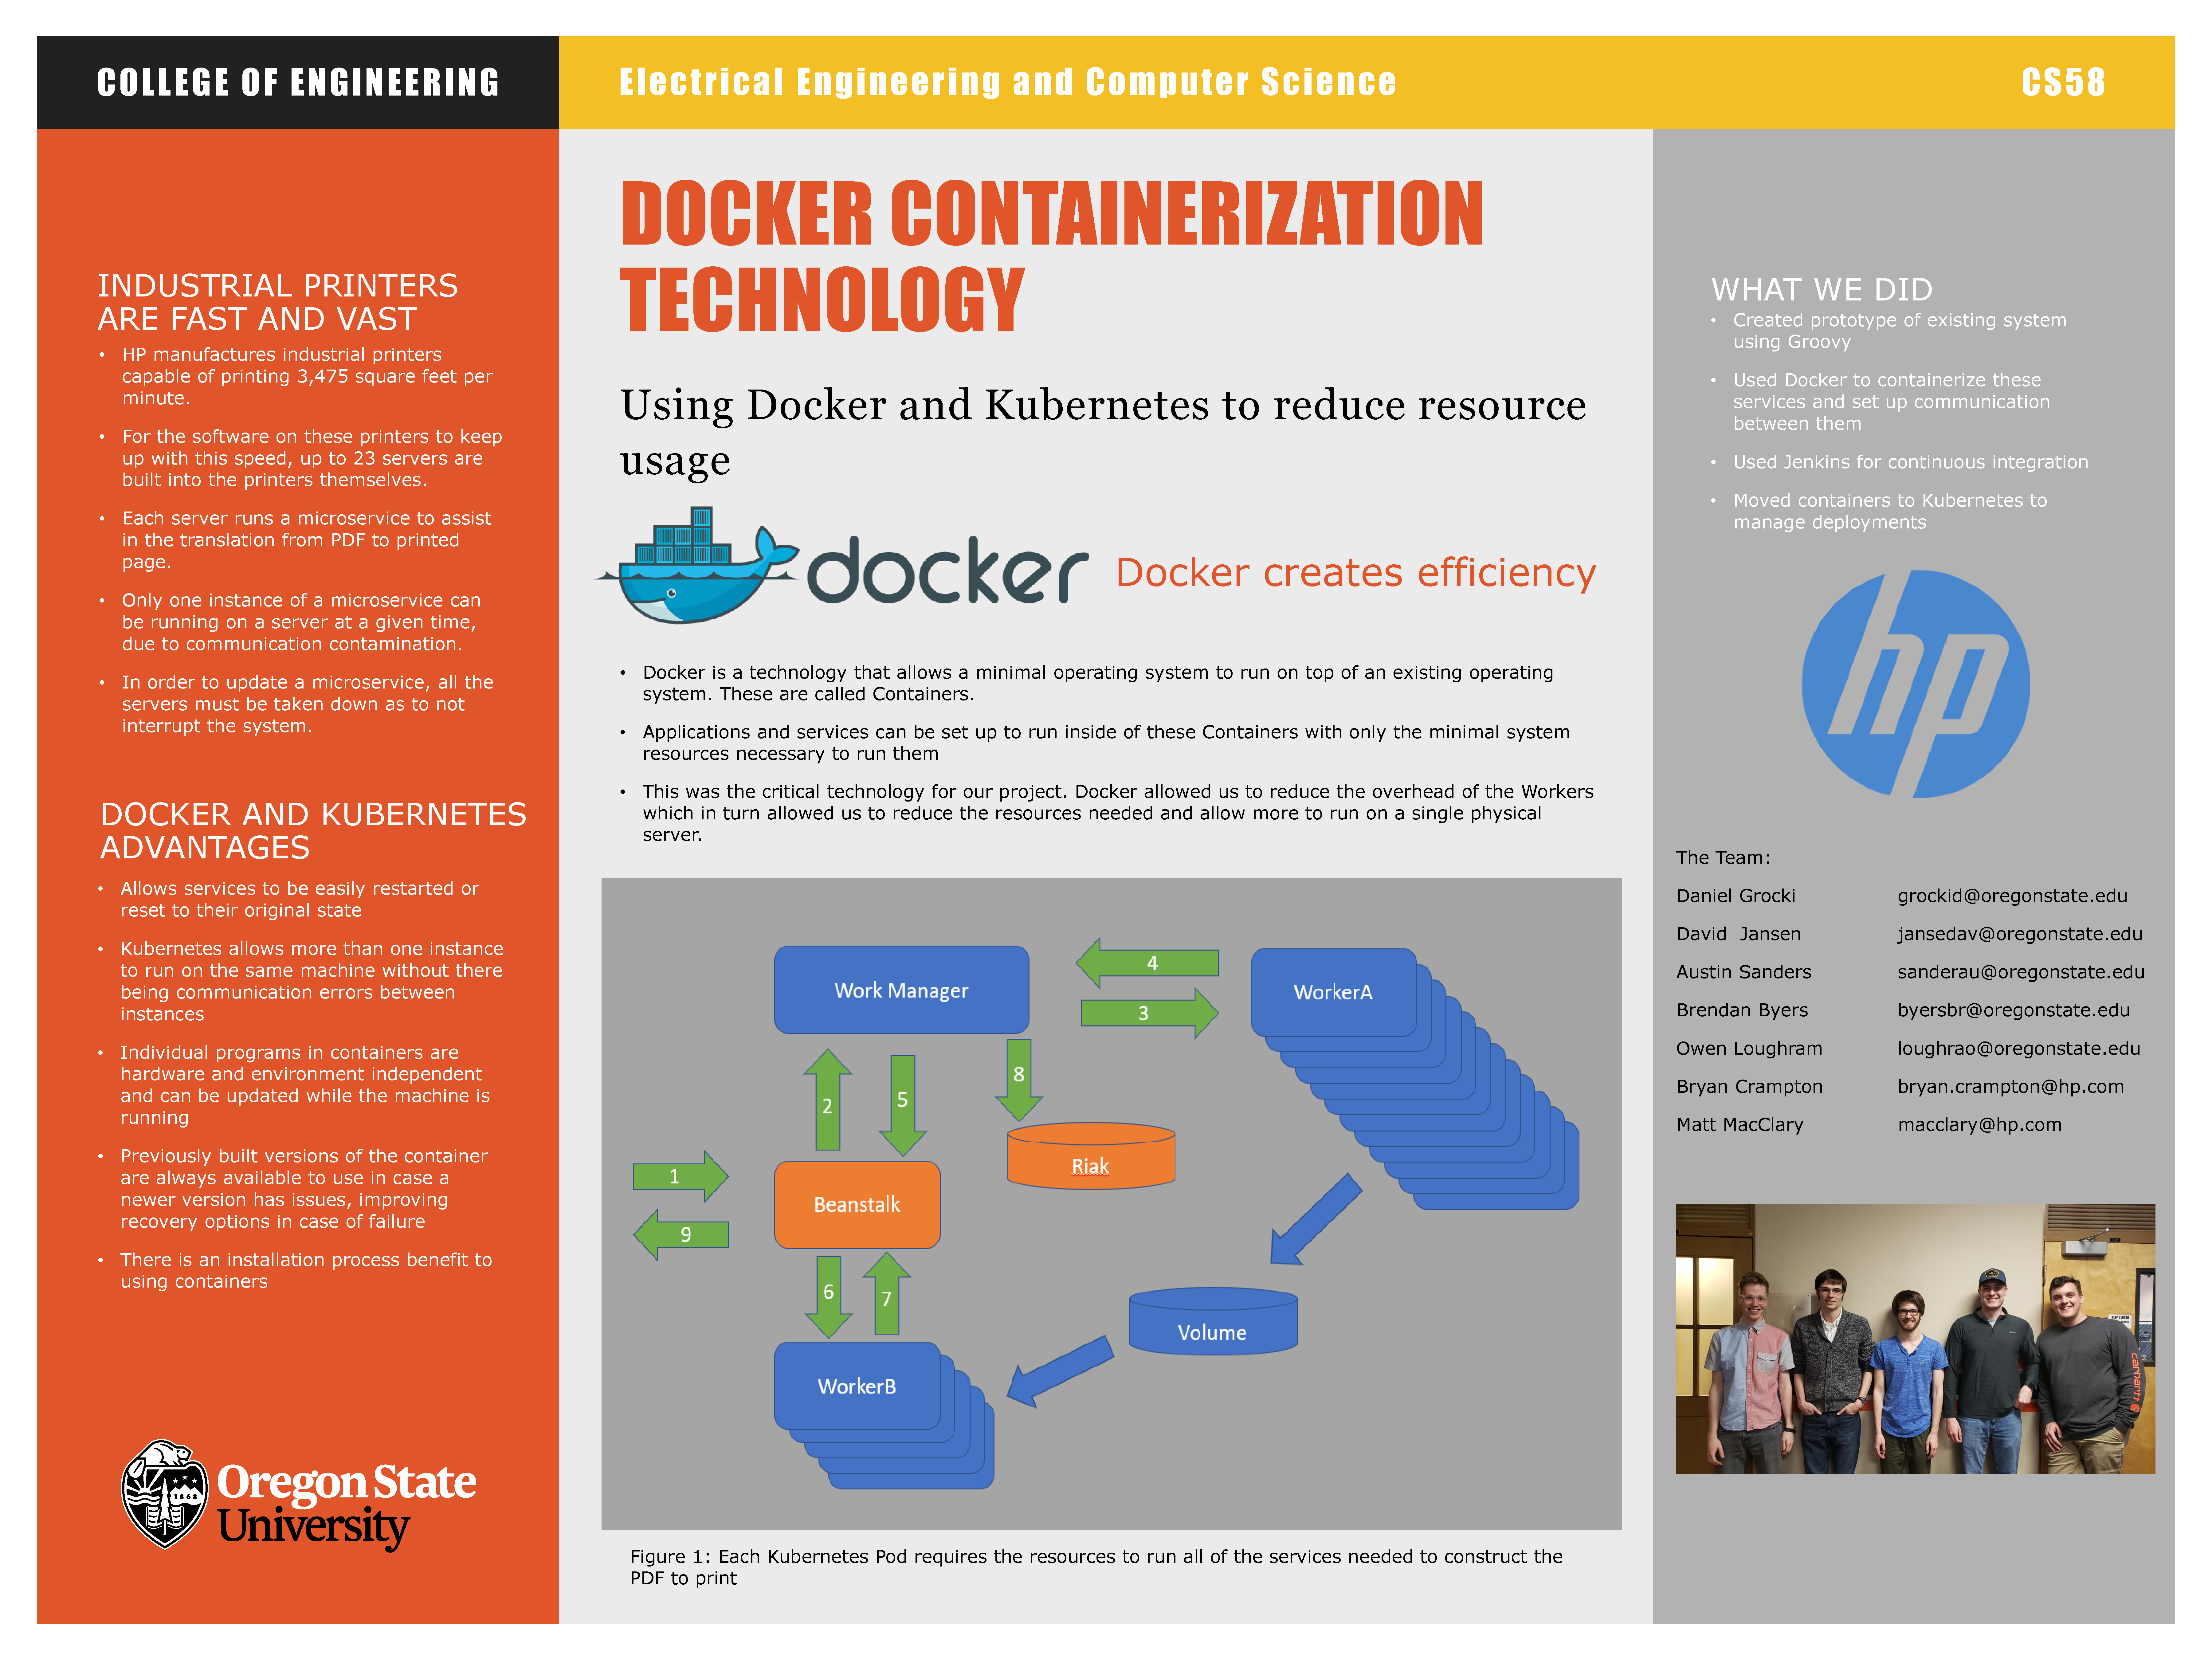
\includepdf[scale =0.9,pages={1},pagecommand=\section{Final Poster}]
{CS_group58_poster_expo_final.pdf}



%%%%%%%%%%%%%%%%%%%%%%%%%%%%%%%%%%%
% Project Documentation
%%%%%%%%%%%%%%%%%%%%%%%%%%%%%%%%%%%
\section{Documentation}

\subsection{Project Architecture}
Our project architecture can be depicted very succinctly with the diagram below. It represents the flow of data, structure of our workers, container isolation, and pod design. The green arrows show the flow of data, the blue and orange rectangles represent Docker containers, and the grey rectangle represents a Kubernetes pod. 
\begin{center}
    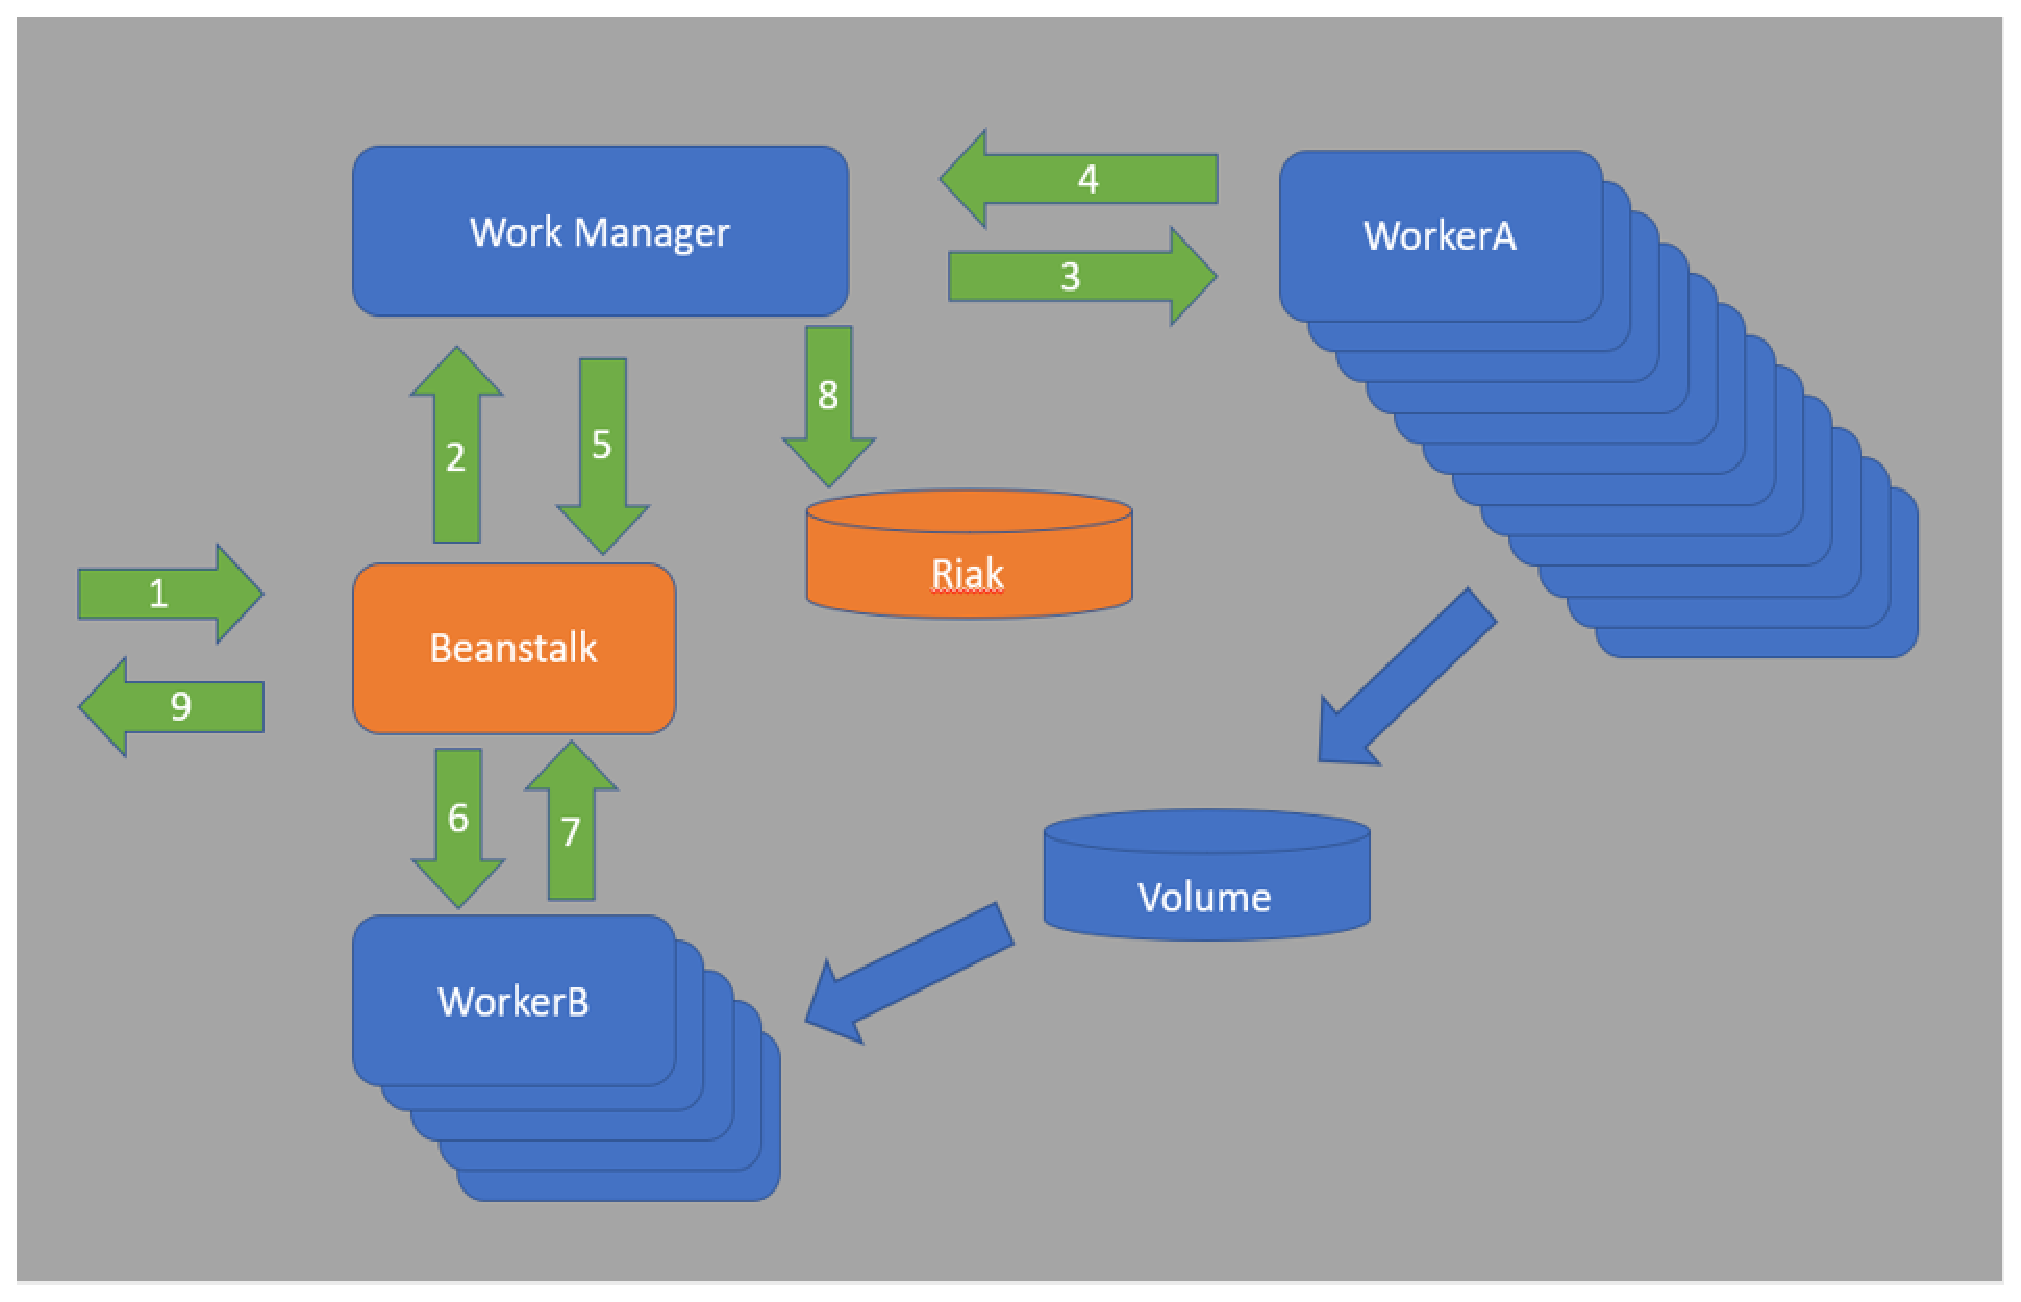
\includegraphics[width=\textwidth, height=10cm]{ProjectFlow.eps}
\end{center}
The dataflow is described as follows:

(1. ) A work job in json format is submitted via http post to the Beanstalk container.

(2. ) The work job is pulled from the beanstalk queue up by the Work Manager.

(3. ) WorkerA is notified via a websocket that there is work to be done, it then will use an HTTP get request to pull the detailed job from the Work Manager. Once it knows the details of the job it will locate the accompanying pdf and perform text insertions.

(4. ) Work Manager is notified via http post that WorkerA has completed its modifications.

(5. ) Work Manager places the job into WorkerB's work queue in Beanstalk.

(6. ) WorkerB pulls the job from its Beanstalk queue, and combines the pdf into 2x2 grids of pages. 

(7. ) WorkerB places the job into back into Work Manager's Beanstalk queue, with a "finsished" flag triggered.

(8. ) Work Manager stores the completed pdf in Riak.

(9. ) The user is provided the pdf Riak ID and location.

\subsection{System Requirements}
Due to Docker and Kubernetes being portable by nature, our project will function on any system that supports these technologies. But, in order to create succinct instructions for installation and deployment the setup guides below require you to be on a CentOS 7 install that is not inside of a virtual machine.

\subsection{Testing and Running Locally}\label{testing-and-running-locally}

To build and test the entire system locally, we will use the scripts
located in \texttt{./MultiTest}.

Once you are in the directory, first setup the work environment by
running \texttt{./setup.sh}. This setup your system for running docker
containers by installing:

\begin{itemize}
\item
  Virtualbox (For minikube)
\item
  Docker
\item
  Docker-Compose
\item
  kubectl
\item
  minikube
\item
  gradlew
\item
  java
\end{itemize}

This will enable you to build the projects from source, run them
locally, and run them in kubernetes.

Once the dependencies are installed, you can test the system locally by
running \texttt{make} or \texttt{make\ setup} from within
\texttt{./MultiTest}. This will download and start the containers needed
to run the system, including:

\begin{itemize}
\item
  Work Manager
\item
  Worker A
\item
  Worker B
\item
  Riak
\item
  Beanstalk
\end{itemize}

To perform a mock request, you can run \texttt{./MakeRequest.sh} or
\texttt{make\ test}. It will use the json present in
\texttt{request.json}, where you can customize filenames of the input
and output PDF's.

To clean up the docker containers and extraneous files after testing,
you can use \texttt{make\ clean}.

\begin{center}\rule{0.5\linewidth}{\linethickness}\end{center}


\subsection{Testing and Running in Kubernetes}\label{testing-and-running-in-kubernetes}

\subsubsection*{Create \texttt{pdf\_io} directory}

First we need to create a directory to hold the pdf input and output of
the system. Create this directory at \texttt{/home}:

\texttt{mkdir\ /home/pdf\_io}

Next add read and write permissions to it with chmod:

\texttt{chmod\ 777\ /home/pdf\_io}

You don't need to use the 777 permission set, we just aren't taking any
chances in these instructions. Just make sure it has read and write
privileges for your user (: ) Next, copy the \texttt{TestPDF.pdf} from
this directory to the \texttt{/home/pdf\_io} directory.

\subsubsection*{Starting the
deployments}\label{starting-the-deployments}

Run the following commands to create the kubernetes pods. If this is the
first time running these commands, it may take upwards of 5 minutes for
them to finish.

Manually: this should be done from the minikube directory

\begin{itemize}
\item
  \texttt{kubectl\ apply\ -f\ riak.yaml}
\item
  \texttt{kubectl\ apply\ -f\ volume.yaml}
\item
  \texttt{kubectl\ apply\ -f\ main.yaml}
\end{itemize}

The system should be ready once all the pods for these deployments are
created. You can check when the deployment is ready

Note: Even after the riak pods are created (member and coordinator) it
takes some time for them to estabilsh the proper connection so the
system make take a minute to work properly even after it says thoes pods
are running.

Now the system should be up and running. The workers pod contains our
entire dockerized system that we wrote in groovy. Those containers are
based off of images that we created and pushed to DockerHub. There
should be 2 sets of workers pods showcasing our ability to create
replicas. To submit a job, do the following:

\subsubsection*{Exec into the python pod to start a
job}\label{exec-into-the-python-pod-to-start-a-job}

There is one pod called python-input. This pod is responsible for
providing a json string of input to beanstalk for the system to work on.
In order to submit a job, we must first enter the python pod.

Run kubectl get pods to get all of the pods that we have created. There
should be one pod called "python-input-\#\#\#\#\#\#\#\#" Copy this
entire pod name.

\texttt{kubectl\ get\ pods}

Next run the following command to exec into the container.

\texttt{kubectl\ exec\ -it\ nameofpodyoucopied\ -\/-\ /bin/bash}

You should now have a prompt in the pod. Type \texttt{ls} to verify that
you can see a script named \texttt{beanstalk\_test.py}.

Run \texttt{beanstalk\_test.py} with python2.7

\texttt{python2.7\ beanstalk\_test.py}

A job has now been submitted. Given 20-30 seconds and there should be a
pdf titled \texttt{Out\_workerspodname.pdf} in your
\texttt{/home/pdf\_io} directory. If there is not, check the
troubleshooting section.

\subsection{Troubleshooting}\label{troubleshooting}

If kubectl does not work, you will need to start the minikube vm. This
is done with the command \texttt{minikube\ start}.

If no files are being created, it may be an issue with the volumes,
check the following. Verify that there is a directory
\texttt{/home/pdf\_io} This directory must have both read and write
permissons. If it doesn't have the permissions, use \texttt{chmod} to
add these permissions. Inside this directory. There should be a PDF
called \texttt{TestPDF.pdf}. If there is not, copy a blank 9 page pdf
into that directory and give it that name. BlankPDF's can be found in
the PDF directory in any of the WorkManager, WorkerA, WorkerB
directories If you don't have read/write permissions on the
\texttt{TestPDF.pdf}, then that could be an issue, trying running chmod
777 on that file

If no Out.pdf is being created (followed by its pod name), but other
files are being added or modified (such as Final.pdf) then there may be
an issue with the riak connection. It is possible that because of the
exception handeling that the workers pods did not properly connect to
the Riak instance due to it not being fully up. To solve this, restart
the workers deployment. This can be done by the following:

\begin{itemize}
\item
  \texttt{kubectl\ delete\ deploy\ workers}
\item
  \texttt{kubectl\ apply\ -f\ main.yaml}
\end{itemize}

Once these pods are up and running then try inputing again

If everything seems to not be working, restart the all deployments:

\texttt{kubectl\ delete\ deploy\ -\/-all}

Then follow manual instructions above.

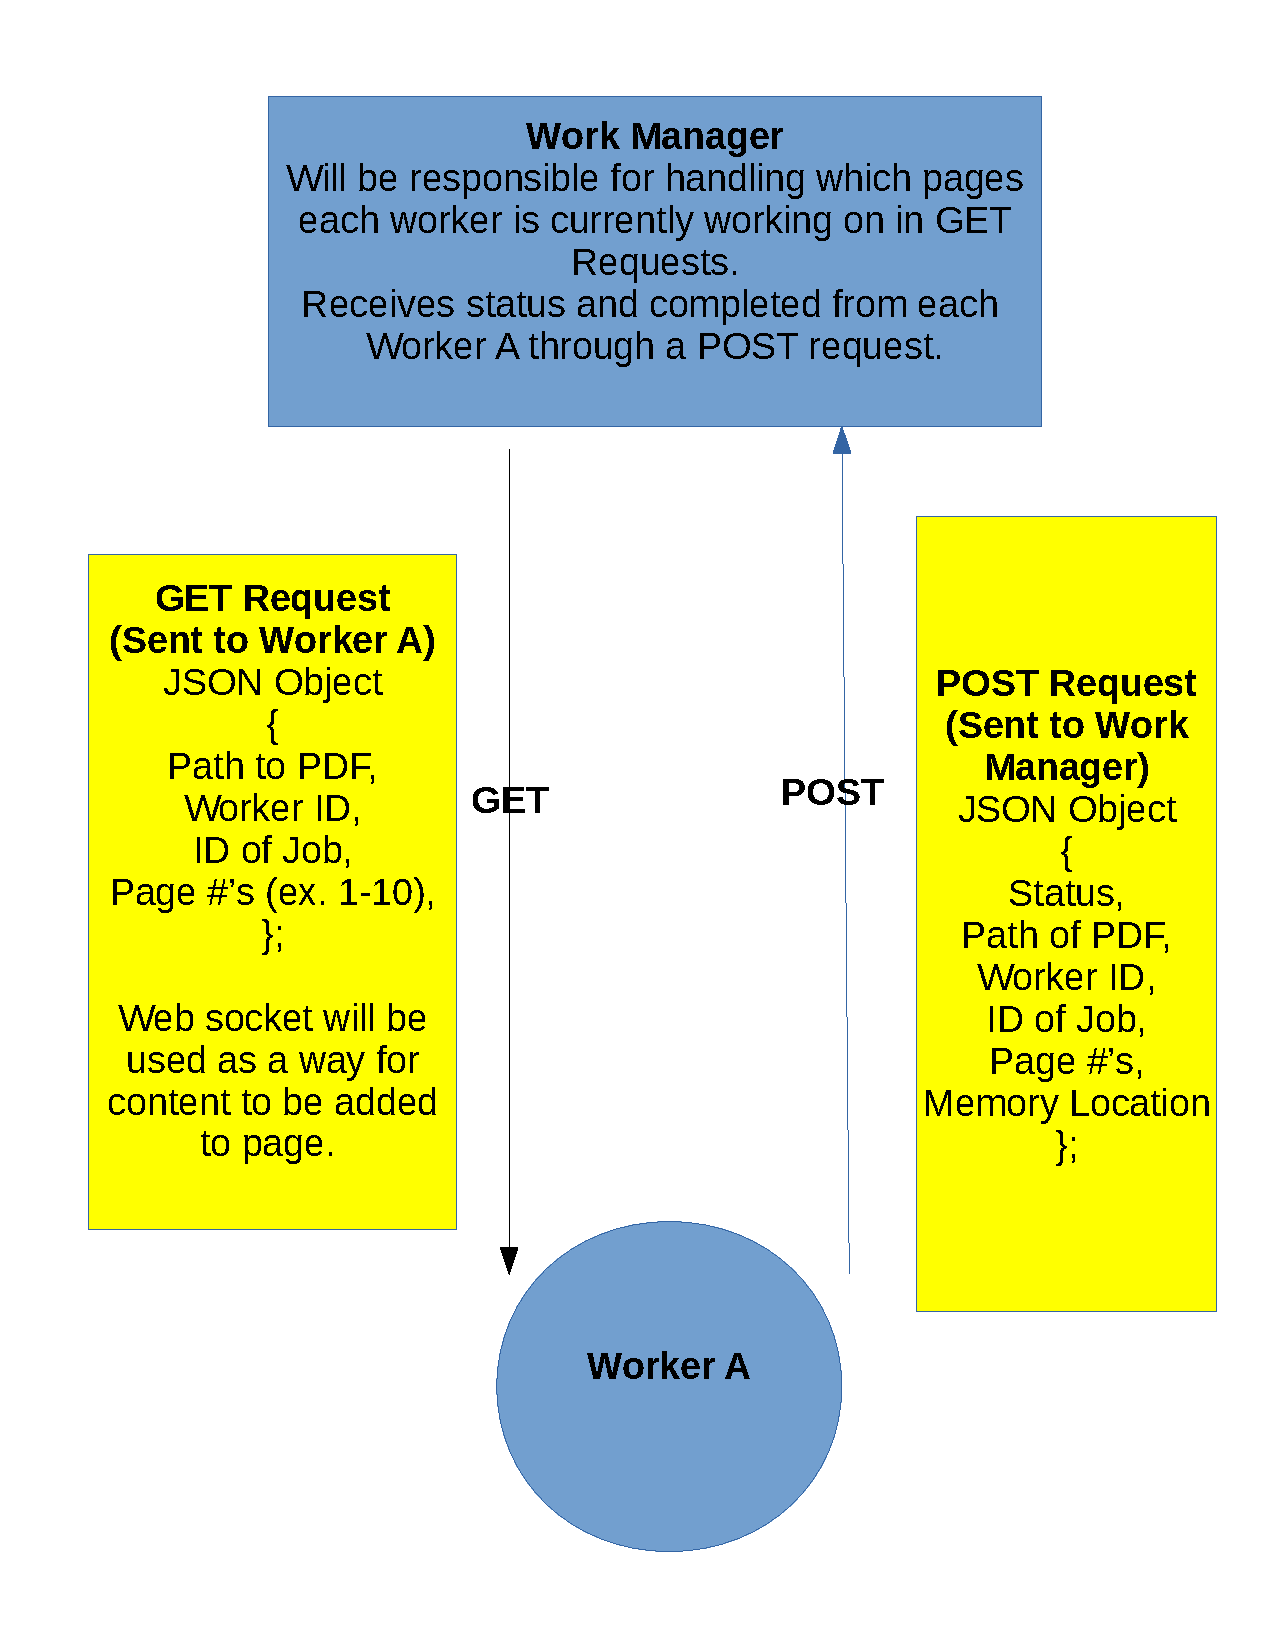
\includepdf[scale=0.8,pages=1,pagecommand={\subsection{API Documentation}}]{WorkerAFinal}
\includepdf[pages=2]{WorkerAFinal}
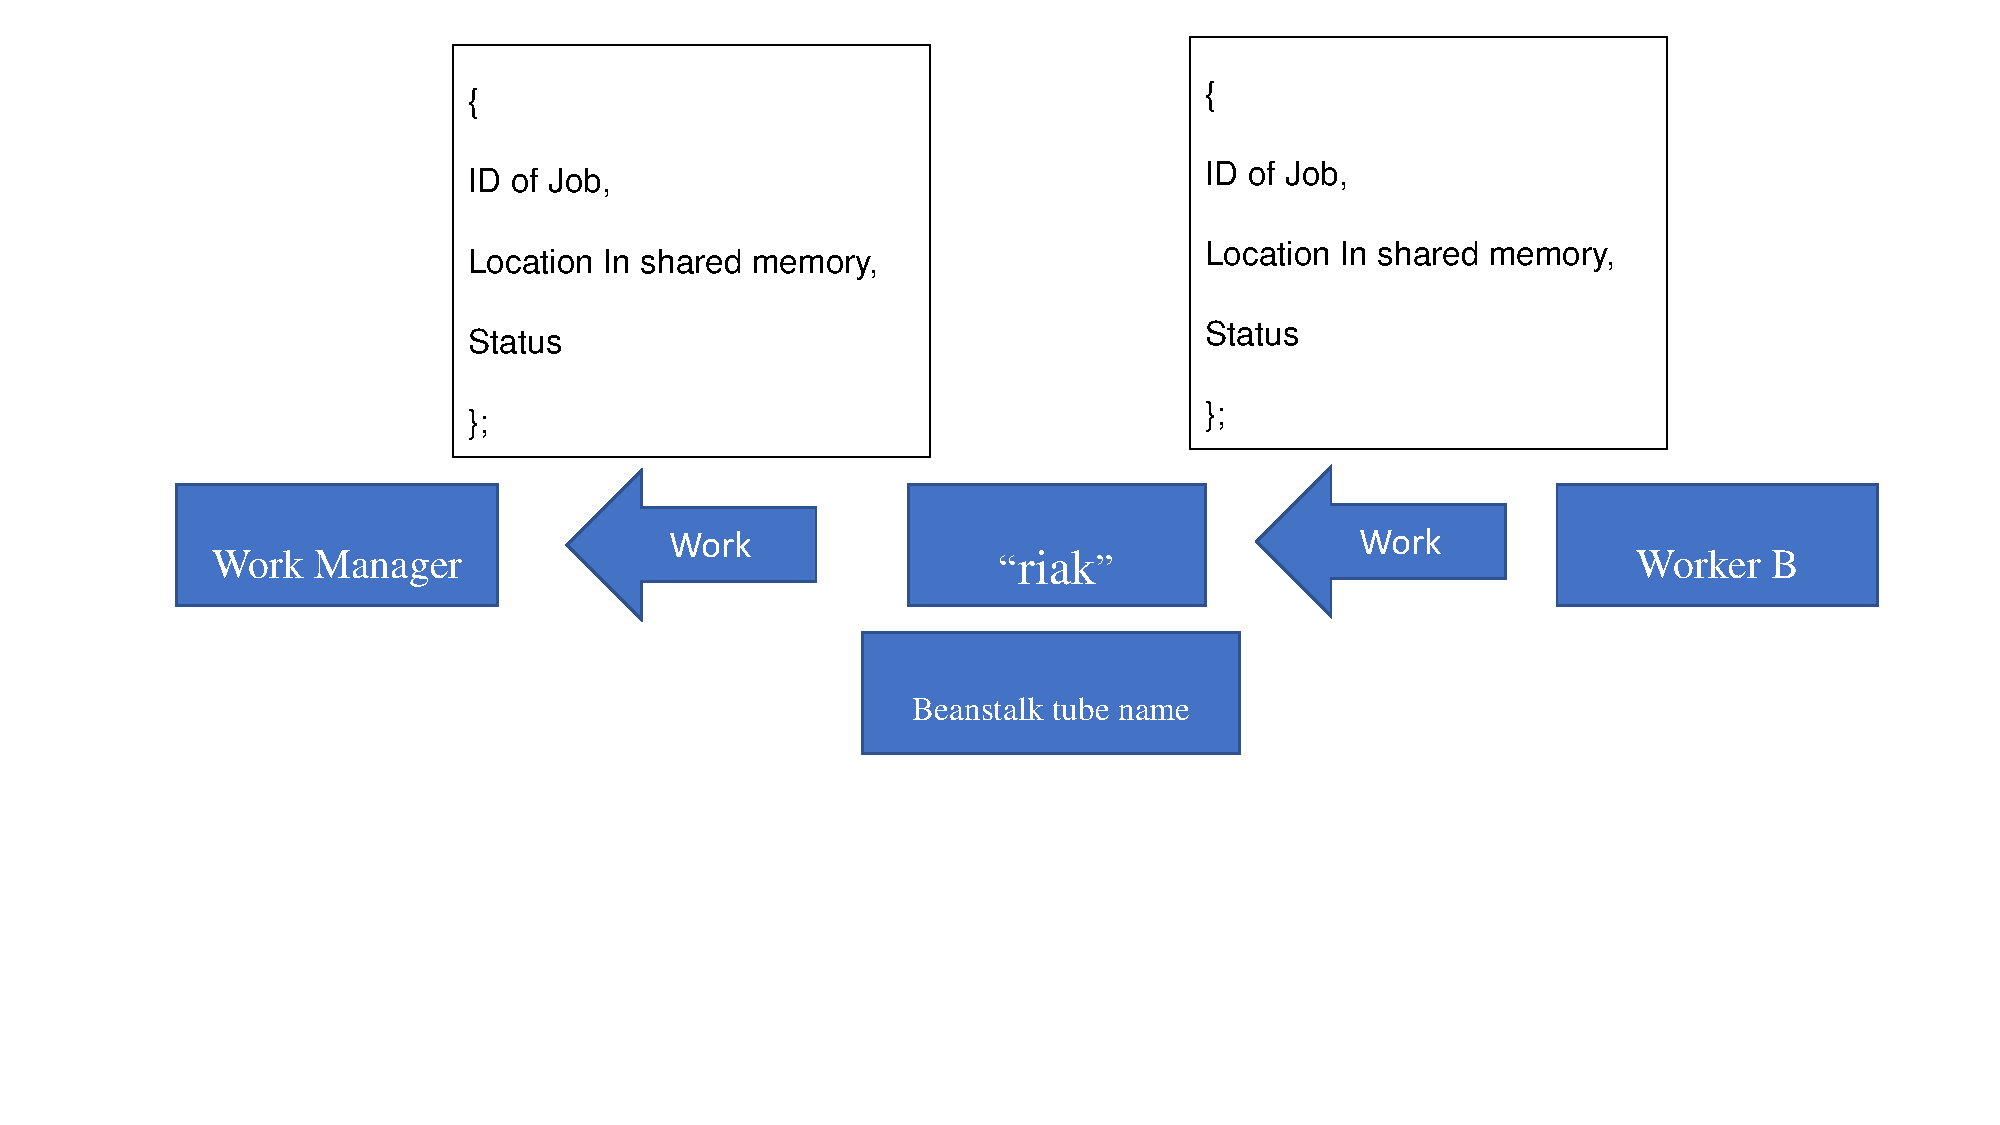
\includepdf[pages=-,nup=1x2]{beanstalk_api_outline}
%%%%%%%%%%%%%%%%%%%%%%%%%%%%%%%%%%
% Recommended Technical Resources
%%%%%%%%%%%%%%%%%%%%%%%%%%%%%%%
\section{Recommended Technical Resources}

\subsection{Helpful Websites}
\subsubsection{Docker}
The Docker website, https://docs.docker.com/, was very helpful during this project. It is a very good resource for Docker information. It explains many different Docker commands as well as how Docker functions. This resource was critical to understanding how to create Docker containers as well as learning to network them together. 
\subsubsection{Kubernetes}
The Kubernetes documentation, https://kubernetes.io/docs/home/, was very helpful to setting up Kubernetes for our project. A large portion of our project was setting up our containers to be successfully deployed in Kubernetes. The Kubernetes Documentation was critical in setting this up. We used this to learn many things, including: setting up minikube, creating Kubernetes deployment files, and working with Kubernetes pods. This is a very important resource to learn more about what can be done with our project in Kubernetes.
\subsubsection{Riak}
The Riak documentation on Docker, https://riak.com/posts/technical/running-riak-in-docker/, was an important resource for our project. This article along with their docs were critical to setting up and understanding the Riak distributed database. We made use of this to help create a Docker Compose file for Riak. 

\subsubsection{Other Resources}
We also gained experience with the technologies we used from classes on Campus. Two classes that stood out were the System Administration class taught by Ben Brewster, and the Cloud Development class taught by Rob Hess.

%%%%%%%%%%%%%%%%%%%%%%%%%%%%%%%%%%%%%%%
% Conclusion
%%%%%%%%%%%%%%%%%%%%%%%%%%%%%%%%%%%%%%
\section{Conclusion}
\subsection{Daniel}
Over the course of this project, I learned a lot of different technical information. I already knew how to use Docker coming in, but I definitely gained more knowledge in this area. I now have I better concept of Docker networks and how containers are able to communicate with each other. I also learned about Kubernetes. I knew what Kubernetes did previously, but this was my first chance to work with it and design a system of deployments using it. This was a great experience and I feel that I have gained a large amount of technical knowledge in this area. 

From a nontechnical view, I learned what it is like to be on a long term team and be a part of a project that is not over in 3 months. I also learned more about how real world code is worked on and deployed to customers. 

As for project work, I learned that it is very important to manage all the aspects of the project. It is important to have a clear understanding of your requirements so that way you can create the product that is asked of you.

I have learned that to have good project management you need to have strong communication and a good schedule of what needs to be done. It is very critical to design beforehand and consider everything before moving forward. When we did design ahead of time, (for example making API diagrams), we had a lot more success then we did not. Managing everything through a clear task list (Agile), is a very efficient way to keep everyone on track and not forget about tasks that need to be done. 

I also learned a good bit about working on a team project. I have been on plenty of team projects before and feel that I work well in a team. But I have never worked in a team with this many people before. Our team worked really well together and had really strong communication. One thing I learned is that on a team of so many people, you have to be assigning tasks to people is very important. Otherwise, it is possible for everyone to think that someone else will be doing something that needs to be done. The use of agile and sprints made this very easy to manage.

If I could do it all over, I would have spent more time talking about the requirements and the outcomes with the team and the clients. I think at times the requirements would change abruptly and we had to adjust to these changes. Another thing I would change would be the focus on Kubernetes and Docker. We spent a lot of time replicating the logic inside HP's system when we likely only needed to model the communication channels. 


\subsection{Owen}
This project served as an excellent way to deepen my knowledge of containerization software and the advantages it can provide. I came into the project with Docker experience and with an understanding of some of the things kubernetes could do. But I quickly had to put this knowledge to the test, we continuously were trying to accomplish new things with docker and creating new containers allowing to get practice and a deeper understanding of the docker technology. While not until the end of the term, the experience with kubernetes was also very beneficial, giving me an understanding of the structure that goes into a system managed by Kubernetes. As far as the other technologies the learning I experienced seemed closer to learning how to do things in groovy, than learning how to do new things.

This was the longest project that I have worked on in my CS career, and it was interesting to see how things work at that scale. I felt like the class was structured in a waterfall way and that would have generally been unbeneficial, but that luckily HP kept us agile and I was able to learn more about story management from that.

Matt and Brian were great at establishing agile practices for us to follow, and in general taught us a lot about how software engineering works in industry. I felt like I had a pretty good understanding of how this worked before the project, but I think it was a valuable experience to see how HP has tailored it to what they believe is best. 

I learned that in project management it is important to establish a consistent understanding of the project across the team before proceeding. The documenetation work we did that was valuable was in plannig our API's and really establishing the flow of data before we began. This is important because it allows developers to work individually without needing others to have completed their tasks first. Each developer can establish their portion alone when things are planned correctly.

I think one of the biggest struggles in this project was appropriately dividing up the work. It was difficult to understand which tasks required what level of effort to complete, and this lead to some tasks not getting completed as quickly as they could have been with proper delegation. Towards the end of the project we learned to help each other out and tackle tasks as a group when they were falling behind.

If I were to do this project again I would try to ensure that we had more freedom on the implementation of the smaller scale pdf ripper. Looking back all we needed was a replication of their communication channels, which we could have busted out quickly in a protyping language. This would have given us more time for the backend of the project and allowed us to go deeper with Kubernetes, or possibly mess with the windows side of things.

\subsection{Austin}

I learned a lot from this project. I don't think I learned any new amazing techniques when it comes to programming, but I think this project taught me how to be a better software engineer and team player. The technical items I learned were how to write in groovy. Which is a like a scripting language and java had a love child. It is a neat language, but has almost documentation so I don't see myself ever using it again unless I am forced to. I learned how to write webservlets. Which was a fun and rewarding experience. I can see myself using this later in my career. I also learned how to use software development tools like gradle. Gradle was a tool I can see myself using again, but I would definitely use an IDE with it if I were to use it again. I also learned about Jenkins and how to write decent unit tests. Mine were to lengthy and unnecessary. The sponsors at HP taught me how to write shorter more comprehensive unit tests. Finally the most useful tool I learned how to use was kubernetes. Kubernetes is a container orchestration tool, and since containerization seems to be the future this seems like a useful skill to learn. I've even had a few jobs I've applied to specifically ask for kubernetes experience which is cool.

The non-technical information I learned is more valuable I think. I learned how to better work inside of a team environment. I learned more about how much time I need to finish projects realistically. Before I would never give myself enough time to finish projects competently, but this project showed me how much time I should actually allocate for each assignment. I also had a more hands on approach to SCRUM cycle which was really cool, and something I will definitely be using in industry.

Project work I learned is taking some big task, and breaking it down into small manageable increments. Its also about learning how to adapt if the goals aren't met or if were are exceeding expectations. If we aren't making dents in an item lets break it down even more. If we are cruising through lets group up items into bigger ticket items. Project work is learning every ones strengths and weaknesses, breaking a task into smaller items, and adapting to change.

What I learned about project management is mostly covered in the project work section. Break a task into smaller items and adapt to unexpected change during production. I would say something that really helped me finish things is when people checked in with me often, and worked together with me to finish items. That is when I really completed the most work during this project.

What I learned about working in teams is that if you do not pull your own weight some one will pick it up for you and it will become obvious. My entire school career I waited till the last few days before something was due to start and finish with it. I worked with team members who were much more proactive, and finish items ahead of time. The began picking up my work, to no fault of their own they just wanted the project done, and I started to look bad because I did not communicate. I learned communication and being proactive with work is key.

If I could do it all over again I think I would just wanted to have worked on the project more. While we completed the project there were some stretch goals I wish I could have met. There was an entire front end to this project that existed inside windows. I think learning containerization and orchestration on windows would have been a useful skill to own. Plus if we completed the front end we would have had an entire working product which would have looked really nice. Instead we just completed the back end which was a great accomplishment, but I just wish I had done more.



\subsection{David}
This project was a great experience for me that taught me a lot. One of the main skills I can take away from this is strong knowledge of the software development life cycle. Matt and Bryan were great with teaching us how software is developed in different stages and what the goal of each stage was. I found this to be very beneficial to me because it will be something I will be doing the rest of my life and this gave me a great introduction for what to expect. I also think that the agile methods they taught us were very valuable, often in interviews I can use this project to showcase important skills like agile that I have experience in. 

Upon entering this project I had a good idea of what Docker was and had even worked on it in the past. Unfortunately I didn't know much of it's uses besides grouping components with their dependencies. After this project I learned many things about containerization, including how you can run multiple duplicate processes on a single server without interference and how easy containerization makes updating components. I believe the skills I learned in Docker will be very beneficial to me in the future especially since I am pursuing a career in web development where it is often used.

My biggest struggle with this project was learning an entirely new programming language and how it worked. We used Groovy for all of our program functionality, at first I didn't even know it was a language. After help from my fellow group mates and a few video tutorials I began figuring out how to work with Groovy. Once I finally realized Groovy was the same as writing Java code without a semicolon things really started clicking for me. Although at first it was a struggle once things started clicking I felt very comfortable in the language and proceeded to build a few good components for our project.

If I were to do this project again I think I would want to change what I worked on. I mainly just did the functionality of the process for this project. Although that helped me learn Groovy I wish I did more of the containerization stuff. The main goal of the project was containerization and I think my focus was more on developing the functionality of the process which ended up taking a lot of time so I didn't have as much time to understand how things were being containerized, especially when it came to the Kubernetes portion of the project.

\subsection{Brendan}
I enjoyed this project because I got to practice many of the skills I've learned in classes to a real project.
I was in charge of much of the behind the scenes work that dealt with building the code.
Once setup, the build server would wait for commits to take place and build the new code.
I have never had to setup anything of this sort before, so it was a great learning experience that I'm sure I can apply in the workforce.
The same goes for docker, where I had basically no knowledge of docker at the beginning.
By the end, I consider myself fairly comfortable with containers, and have started using them for my own projects.

As for non-technical learning, I found how important it is to have clear avenues of communication.
For our group, we had a slack work space for communication with HP and one for communication between each other.
The HP slack made it easy to communicate with the project leads and coordinate where and when we were meeting.
The group-only slack allowed us to communicate more class related happenings with each other like meeting up to work or upcoming assignments.

Project work is much better when the project takes place over a longer time scale.
Because it was done over a 9 month period, it gave me a chance to really learn the technologies and become comfortable with the system.
The short projects in classes are difficult because you never really know the other members, and don't have a lot of time to get to know each other.
The length and scale of this project allowed us to get to know each other much better, making it much more of a team effort than a regular project.
The project was also large enough that all members had a portion of the project that they owned and were in charge of.

It was also different having project leads from HP direct the project instead of just working with teammates.
They have much more development experience than any of us do and helped plan out how the development should operate.
With their guidance and knowledge of the system it made it much easier to create our project mirroring it.

If I were to do the project again, the first thing I would focus on is getting the build and configuration system setup.
One issue I had was that docker and jenkins were implemented in the different workers after they had already been completed.
There were a few issues with how the code was built and packaged that caused issues with Jenkins.
By having a jenkins and docker foundation already setup before starting to code, it would have made it easier to incorporate the different workers into build pipelines.

\clearpage
%%%%%%%%%%%%%%%%%%%%%%%%%%%%%%%
%References
%%%%%%%%%%%%%%%%%%%%%%%%%%%%%%%
\bibliographystyle{ieeetr}
\bibliography{references}



\clearpage

%%%%%%%%%%%%%%%%%%%%%%%%%%
%Appendix
%%%%%%%%%%%%%%%%%%%%%%%%%
\begin{appendices}


\section{Kubernetes YAML}
\begin{lstlisting}[language=java]
#Beanstalk deployment 
apiVersion: apps/v1
kind: Deployment
metadata:
  name: beanstalk-deployment
  namespace: default
  labels:
    app: beanstalk
spec:
  replicas: 1
  selector:
    matchLabels:
      app: beanstalk
  template:
    metadata:
      labels:
        app: beanstalk
    spec:
      containers:
      - name: beanstalk
        image: schickling/beanstalkd:latest
        ports:
        - containerPort: 11300
---
#Beanstalk Service
kind: Service
apiVersion: v1
metadata:
  name: beanstalk 
spec:
  selector:
    app: beanstalk
  ports:
  - protocol: TCP
    targetPort: 11300
    port: 11300 
  type: LoadBalancer
---

#WorkManager and WorkerA
apiVersion: apps/v1
kind: Deployment
metadata:
  name: workers
  labels:
    app: workmanager
spec:
  replicas: 2
  selector:
    matchLabels:
      app: workmanager
  template:
    metadata:
      labels:
        app: workmanager
    spec:
      containers:
      - name: workmanager
        image: dgrocki/workmanager:latest
        volumeMounts:
        - name: wm-vol
          mountPath: "/mnt"
        env:
          - name: POD_NAME
            valueFrom:
              fieldRef:
                fieldPath: metadata.name


      - name: workera1
        image: dgrocki/workera:latest
        volumeMounts:
        - name: wm-vol
          mountPath: "/mnt"
        env:
          - name: POD_NAME
            valueFrom:
              fieldRef:
                fieldPath: metadata.name
      - name: workera2
        image: dgrocki/workera:latest
        volumeMounts:
        - name: wm-vol
          mountPath: "/mnt"
        env:
          - name: POD_NAME
            valueFrom:
              fieldRef:
                fieldPath: metadata.name



      - name: workerb1
        image: dgrocki/workerb:latest
        volumeMounts:
        - name: wm-vol
          mountPath: "/mnt"
        env:
          - name: POD_NAME
            valueFrom:
              fieldRef:
                fieldPath: metadata.name
      - name: workerb2
        image: dgrocki/workerb:latest
        volumeMounts:
        - name: wm-vol
          mountPath: "/mnt"
        env:
          - name: POD_NAME
            valueFrom:
              fieldRef:
                fieldPath: metadata.name
      volumes:
      - name: wm-vol 
        persistentVolumeClaim:
          claimName: shared-memory1
#---
#kind: Service
#apiVersion: v1
#metadata:
#  name: workmanager 
#spec:
#  selector:
#    app: workmanager 
#  ports:
#  - protocol: TCP
#    port: 8080
#  type: LoadBalancer
---
apiVersion: apps/v1
kind: Deployment
metadata:
  name: python-input
  labels:
    app: py 
spec:
  replicas: 1
  selector:
    matchLabels:
      app: py 
  template:
    metadata:
      labels:
        app: py 
    spec:
      containers:
      - name: py
        image: dgrocki/beanstalk-input:latest
        command:
        - /bin/sh
        - "-c"
        - "sleep 60m"
\end{lstlisting}
\clearpage
\section{Beanstalk Class}
\begin{lstlisting}[language=java]

class BeanstalkClient{
	//private ClientImpl connection = new ClientImpl("0.0.0.0", 11300);
	private String pod_id;
	private ClientImpl connection;
	private JobImpl currentJob;	//can we only be working on one job at a time?
	private String riak;
	private String worker_b;
	private String status;

	public BeanstalkClient(){
		pod_id = System.getenv("POD_NAME");
		println pod_id;
		connection  = new ClientImpl("beanstalk", 11300); 
		riak = "riak" + pod_id;		
		worker_b = "to_worker_b" + pod_id;
		status = "status" + pod_id;
	}

	public List<String> listTubes(){
				
		return connection.listTubes();
	}

	public void sendWork(String json){
		long priority = 0;
		int delaySeconds = 0;
		int timeToRun = 10;
		byte[] data = json.getBytes();

		connection.put(priority, delaySeconds, timeToRun, data);
	}	
	//functionhere for testing purposes
	public void useTube(String s){
		connection.useTube(s);
	}
	//pull a new job off the new_work queue
	public String recieve_new_work(){
		connection.watch("new_work");
		JobImpl job = connection.reserve();
		String s = new String(job.data);
		connection.delete(job.jobId);
		return s;
	}

        // Send work to workerA
        public void send_to_workerA(String json) {
            connection.useTube("new_work");
            sendWork(json);
        }

	//put a new job on the to_workerB queue
	public void send_to_workerB(String json){
		connection.useTube(worker_b);
		sendWork(json);
		
		
	}
	//pull a job off of the riak queue
	//returns a string of json data and the job is deleted
	public String recieve_riak_work(){

		connection.watch(riak);
		JobImpl job = connection.reserve();
		String s = new String(job.data);
		connection.delete(job.jobId);
		return s;

	}
	//put a job on the status queue
	public void send_status(String json){
		connection.usetTube(status);
		sendWork(json);
	}

        public boolean peek_jobs() {
                String resp = connection.peek()

                if(resp == "NOT_FOUND\r\n") {
                    return false;
                } else {
                    return true;
                }
        }



}

\end{lstlisting}

\clearpage
\section{WorkManager}
\begin{lstlisting}[language = java]
class WorkManager{

	public static void main(String [] args) {



		def riak = actor{
			BeanstalkClient beanstalk = new BeanstalkClient();		

			Riak riak_client = new Riak();
			while(1){
				String new_work = beanstalk.recieve_riak_work();
				def parser = new JsonSlurper();
				def data = parser.parseText(new_work);

				println data;	
				String s = data.outPath;

				println s;

				File file = new File(s);
				byte[] fileArray;
				fileArray = Files.readAllBytes(file.toPath());


				println "Storing in riak... ";
				riak_client.store(fileArray);
				


				println "Fetching from riak... ";
				byte[]fetch =  riak_client.fetch();
				//println fetch;
				String pod_id = System.getenv("POD_NAME");
				println pod_id;
				s = "/mnt/Out_" + pod_id + ".pdf";
				File file2 = new File(s);
				Files.write(file2.toPath(), fetch);

				if(fetch != fileArray){
					println "false";
					println "1" + fileArray.length;
					println "2" + fetch.length;
				}else{println "true";}
				
			}

		}

		def await_new_work = actor {
			BeanstalkClient beanstalk = new BeanstalkClient();		
			beanstalk.useTube("new_work");
			final Jetty jetty = new Jetty(8080, beanstalk);
			println "jetty made"
			jetty.start();
			println "jetty started"
			Thread.sleep(500);
			if (false == jetty.isStarted()) {
				throw new Exception("Cannot start jetty server");
			}

		}


		//setup all the threads
		[riak, await_new_work]*.join()

			return;
	}

}
\end{lstlisting}


\end{appendices}
\end{document}